\documentclass[10pt,table,mathserif]{beamer}
\usetheme[
%%% options passed to the outer theme
%    hidetitle,           % hide the (short) title in the sidebar
%    hideauthor,          % hide the (short) author in the sidebar
%    hideinstitute,       % hide the (short) institute in the bottom of the sidebar
%    shownavsym,          % show the navigation symbols
%    width=2cm,           % width of the sidebar (default is 2 cm)
%    hideothersubsections,% hide all subsections but the subsections in the current section
%    hideallsubsections,  % hide all subsections
%    right                % right of left position of sidebar (default is right)
  ]{Aalborg}

\setbeamertemplate{theorems}[numbered]

\definecolor{watred}{cmyk}{.00,1,1,0.00}
\definecolor{watyellow}{cmyk}{0,0.12,1,0}
\definecolor{watgray}{cmyk}{0,0,0,0.5}

% If you want to change the colors of the various elements in the theme, edit and uncomment the following lines
% Change the bar and sidebar colors:
\setbeamercolor{Aalborg}{fg=black,bg=watred}
\setbeamercolor{sidebar}{bg=white}
% Change the color of the structural elements:
\setbeamercolor{structure}{fg=red}
% Change the frame title text color:
%\setbeamercolor{frametitle}{fg=blue}
% Change the normal text color background:
\setbeamercolor{normal text}{bg=white, fg=black}
\setbeamercolor{alerted text}{bg=white, fg=red}
% ... and you can of course change a lot more - see the beamer user manual.
\usepackage{xcolor}
\usepackage[utf8]{inputenc}
\usepackage[english]{babel}
\usepackage[T1]{fontenc}
\usepackage{threeparttable}
% ... or whatever. Note that the encoding and the font should match. If T1
% does not look nice, try deleting the line with the fontenc.
\usepackage{lmodern} 
\usepackage{subfigure}
\usepackage{algorithm}
\usepackage{algorithmic}
\usepackage{colortbl}
\usepackage{biblatex}
\usepackage{bibentry}
\usepackage{epstopdf}
\usepackage{caption}
\usepackage{multirow}

\usepackage{tikz}
\usetikzlibrary{shapes}
\usetikzlibrary{arrows}
\usetikzlibrary{positioning, fit, arrows.meta}
\usepackage{tkz-graph}
\usetikzlibrary{backgrounds,automata}
\bibliography{mybib.bib}



\newcommand*{\Scale}[2][4]{\scalebox{#1}{$#2$}}%
\newcommand*{\Resize}[2]{\resizebox{#1}{!}{$#2$}}%
\newcommand{\vt}[1]{\mathbf{#1}}
\newcommand{\vw}{\mathbf{w}}
%\newcommand{\pm}{\stackrel{+}{-}}
\newcommand{\vx}{\mathbf{x}}
\newcommand{\vi}{\mathbf{i}}
\newcommand{\vo}{\mathbf{o}}
\newcommand{\vxt}{\tilde{\mathbf{x}}}
\newcommand{\vy}{\mathbf{y}}
\newcommand{\impsigma}{\breve{\sigma}}
\newcommand{\barK}{\overline{K}}
\newcommand{\barC}{\overline{C}}
\newcommand{\vz}{\mathbf{z}}
\newcommand{\fnp}{\tilde{f}}
\newcommand{\vu}{\mathbf{u}}
\newcommand{\vs}{\mathbf{s}}
\newcommand{\vc}{\mathbf{c}}
\newcommand{\E}{\mathbf{E}}
\newcommand{\HK}{\mathcal{H}_K}
\newcommand{\XS}{\mathcal{X}}
\newcommand{\DS}{\Delta S}
\newcommand{\Heston}{\textsc{Heston}}
\newcommand{\DVmkt}{\Delta \breve{V}}
\newcommand{\DT}{\Delta_t}
\newcommand{\vuu}{\mathbf{\widetilde u}}
\newcommand{\Real}{\mathbb{R}}
\newcommand{\vdot}[2]{{#1}^T{#2}}
\DeclareMathOperator*{\argmin}{\arg\!\min}
\newcommand{\sym}{\textsc{sym}}
\newcommand{\BS}{\textsc{BS}}
\newcommand{\LOF}{\textsc{lof}}
\newcommand{\svm}{\textsc{svm}}
\newcommand{\AMflag}{\text{mFLAG}}
\newcommand{\rw}{\textsc{rw}}
\newcommand{\diag}{\textsc{diag}}
\newcommand{\sign}{\textsc{sign}}
\newcommand{\MeanAbs}{\E(|\DVmkt-\DS f(\vx)|)}
\newcommand{\Cluster}{\textsc{C}}
\newcommand{\bi}{\text{bi}}
\newcommand{\g}{\mathbf{g}}
\newcommand{\vv}{\mathbf{v}}
\newcommand{\valpha}{\pmb{\alpha}}
\newcommand{\vK}{\pmb{K}}
\newcommand{\vV}{\pmb{\breve{V}}}
\newcommand{\e}{\mathbf{e}}
\newcommand{\vol}{\upsilon}
\newcommand{\vd}{\mathbf{d}}
\newcommand{\vh}{\mathbf{h}}
\newcommand{\vf}{\mathbf{f}}
\newcommand{\vW}{\pmb{W}}
\newcommand{\np}{\text{np}}
\newcommand{\pt}{^{+\Delta t}}
\newcommand{\norm}{\text{norm}}
\newcommand{\row}{\text{row}}
\newcommand{\Vmkt}{\breve{V}}
\newcommand{\vecVmkt}{\mathbf{\breve{V}}}
\newcommand{\Ncut}{\text{Ncut}}
\newcommand{\half}{\frac{1}{2}}
\newcommand{\DKLs}{\bf\textsc{DKL}_{\text{SPL}}}
\newcommand{\DKLg}{\bf\textsc{DKL}_{\text{RBF}}}
\newcommand{\IKLs}{\bf\textsc{IKL}_{\text{SPL}}}
\newcommand{\IKLg}{\bf\textsc{IKL}_{\text{RBF}}}
\newcommand{\LVF}{\textsc{LVF}}
\newcommand{\Del}{\delta^{\textsc{BS}}}
\newcommand{\SABR}{\bf\textsc{SABR}}
\newcommand{\MV}{\bf \textsc{MV}}
\newcommand{\vU}{\pmb{U}}
\newcommand{\vb}{\mathbf{b}}




\nobibliography{Ref.bib}
\definecolor{mycyan}{cmyk}{.2,0,0,0}
\definecolor{mycyan1}{cmyk}{.1,0,0,0}
\definecolor{mycyan3}{cmyk}{.3,0,0,0}
% colored hyperlinks
\newcommand{\chref}[2]{%
  \href{#1}{{\usebeamercolor[bg]{Aalborg}#2}}
}

\title[Data-Driven Models for Discrete
Hedging Problem ]% optional, use only with long paper titles
{Data-Driven Models for   Discrete
Hedging Problem}


\author[Ke Nian ] % optional, use only with lots of authors
{ Ke Nian\\
 Supervisors: Prof.Yuying Li and Prof.Thomas.F.Coleman
}


% - Give the names in the same order as they appear in the paper.
% - Use the \inst{?} command only if the authors have different
%   affiliation. See the beamer manual for an example

%specify some optional logos
\pgfdeclareimage[height=1.4cm]{mainlogo}{logo.png} % placed in the upper left/right corner
\logo{\pgfuseimage{mainlogo}}

\pgfdeclareimage[height=0.75cm]{logo2}{tu-logo} % placed in the lower left/right corner if the \pgfuseimage{logo2} command is uncommented in the \institute command below

\institute[
%  {\pgfuseimage{logo2}}\\ %insert a company or department logo
  David R. Cheriton School of Computer Science, University of Waterloo
] % optional - is placed in the bottom of the sidebar on every slide
{%
  David R. Cheriton School of Computer Science,\\
  University of Waterloo,\\
  Waterloo, Canada
  %there must be an empty line above this line - otherwise some unwanted space is added between the university and the country (I do not know why;( )
}
\date{\today}

\begin{document}
% the titlepage
\begin{frame}[plain] % the plain option removes the sidebar and header from the title page
  \titlepage
\end{frame}
%%%%%%%%%%%%%%%%

% TOC
\begin{frame}{Agenda}{}
\tableofcontents
\end{frame}
%%%%%%%%%%%%%%%%

\section{Introduction}


\begin{frame}{Practitioner Black-Scholes (BS) Delta Hedging}

\begin{itemize}
  \item BS model:
\[
\frac{d S}{ S}= \mu dt +\sigma dZ
\]

\[
\sigma:\; \text{Constant}
\]
\item Implied Volatility
  \[
  \sigma_{imp}=V_{BS}^{-1}(V_{mkt},.)
  \]
  \begin{center}
  $V_{mkt}$: market option price \\ $V_{BS}^{-1}$ : inverse of BS pricing function
  \end{center}

\item BS Delta:
\[
\delta_{BS}=\frac{\partial V_{BS}}{ \partial S}
\]
\end{itemize}

\end{frame}






\begin{frame}{Problem with Black-Scholes Delta}
Problem with the traditional Black-Scholes delta:
\begin{itemize}
  \item Market violates BS assumption
  \item Dependence of volatility on underlying asset price
\end{itemize}
Variants of Hedging Strategy:
\begin{itemize}
  \item Stochastic Volatility Model
  \item Local Volatility Model
  \item Minimum Variance Approach
  \item Indirect Data-Driven Approach
  \item \textbf{Direct Data-Driven Approach}
\end{itemize}
\end{frame}
\section{Delta Hedging Variants}
\subsection{Stochastic Volatility Model}
\begin{frame}{Stochastic Volatility Model}
Stochastic volatility models:
\begin{itemize}
  \item Heston Model
\[
\begin{split}
dS_t&=r S_t dt + \sqrt{\upsilon_t} S_t dW_t\\
d\upsilon_t&=\kappa(\overline{\upsilon}-\upsilon_t)dt+\eta \sqrt{\upsilon_t}dZ_t\\
dZ_tdW_t&=\rho dt
\end{split}
\]
\item Many stochastic volatility models do not have analytical formula for pricing and hedging function.
\end{itemize}
\end{frame}



\subsection{Minimum Variance Approach}
\begin{frame}{Minimum Variance Approach}
Considering the  the dependence of imply volatility on asset price:
\begin{itemize}
\item The  Minimum Variance (MV) delta:
\[
\delta_{MV}=\frac{\partial V_{BS}}{\partial S}+\frac{\partial V_{BS}}{\partial \sigma_{imp}}\frac{\partial \sigma_{imp}}{ \partial S}
\]
\item The authors \footnotemark propose:
\begin{equation}
\frac{\partial \sigma_{imp}}{ \partial S}=\frac{a+b\delta_{BS}+c \delta_{BS}^2}{S\sqrt{T}}
\end{equation}
$a, b \text{ and  } c$ are the parameter to be fitted using market data.
\end{itemize}
\footnotetext[1]{Hull, J. and White, A., "Optimal delta hedging for options."
\\Journal of Banking  and  Finance 82 (2017): 180-190.}
\end{frame}

\subsection{Local Volatility Model}
\begin{frame}{Local Volatility Model}
The local volatility function (LVF) \footnotemark : volatility is a deterministic function of $S$ and $t$.
 \[
\delta_{MV}=\frac{\partial V_{BS}}{\partial S}+\frac{\partial V_{BS}}{\partial \sigma_{imp}}\frac{\partial \sigma_{imp}}{ \partial S}
\]
Local volatility model can also be used to calculate the $\frac{\partial \sigma_{imp}}{ \partial S}$.

\footnotetext[2]{Coleman, T.F., Kim, Y., Li, Y. and Verma, A.,\\ 'Dynamic hedging with a deterministic local volatility function model,' \\Journal of risk, 4 ,1 (2001):63-89}

\end{frame}
\section{Data Driven Approach}
\subsection{Indirect Data-Driven Approach}
\begin{frame}{Problem with Parametric Approach}
Parametric approaches:
\begin{itemize}
  \item Model mis-specification.
  \item Sub-optimal for discrete hedging problems.
\end{itemize}

Data-driven approaches:.
\begin{itemize}
  \item Minimum assumptions on $S$.
  \item Model is determined by market data.
\end{itemize}


\end{frame}


\begin{frame}{Indirect Data-driven Approach}
The indirect data-driven approach \footnotemark can be summarized as following:
\begin{itemize}
\item Let $X$ be the features from market.
\begin{itemize}
  \item Asset price $S$
  \item Strike Price $K$
  \item Time to expiration $T-t$
\end{itemize}
\item Determine the data driven pricing function $V(X)$ using regression model.
\item Compute
\[
\delta_{ID}=\frac{ \partial V(X) }{ \partial S}
\]
\end{itemize}
\footnotetext[3]{Hutchinson, J.M., Lo, A.W. and Poggio, T., "A \\
nonparametric approach to pricing and hedging derivative securities via learning networks." The Journal of Finance 49.3 (1994): 851-889.}
\end{frame}

\subsection{Direct Data-Driven Approach}
\begin{frame}{Problem with Indirect Data-Driven Approach}
Problem with the Indirect Data-Driven Approach:
\begin{itemize}
  \item Unnecessary intermediate procedure.
  \item Sub-optimal for discrete hedging.
  \item Model parameters depend on the asset price.
\end{itemize}

Direct data-driven approach can be more useful in practice.
\begin{itemize}
  \item Customized hedging position function.
  \item Directly compute the hedging position.
\end{itemize}
\end{frame}

\begin{frame}{Direct Data-driven Approach}

The direct data-driven approach is
\[
\min_{f}\left[\frac{1}{N} \sum_{i=1}^N (\Delta V_i-\Delta S_i f(X_i))^2 \right]
\]

\begin{center}
$\Delta V_i$ : the change of option value in data instance $i$\\
$\Delta S_i$ : the change of asset price in data instance $i$ \\
\end{center}
\end{frame}



\subsection{Real Data Experiments}
\begin{frame}{Real Data  Hedging Experiments}
\begin{itemize}
  \item Data: S\&P 500 index option from Jan 2007 and Aug 2015
  \item Model Calibration:
    \begin{itemize}
      \item SABR: daily calibration
      \item LVF: $\frac{\partial \sigma_{imp}}{ \partial S}$ from implied volatility surface
      \item MV: Use a 36 months time window to train
      \item $\DKLs$: Use a 36 months time window to train. Models are separately calibrated for different Black-Sholes delta range.
    \end{itemize}
  \end{itemize}
\end{frame}

\begin{frame}{Evaluation Criteria: Local Risk}
The percentage increase in the effectiveness over the BS hedging:
\[
Gain=1-\frac{SSE[\Delta V_i-\Delta S_i\delta^i]}{SSE[\Delta V_i-\Delta S_i\delta^i_{BS}]}
\]
\begin{center}

SSE: sum of squared errors\\
 $\delta$: hedging position computed from different models\\
 $\delta_{BS}$: BS delta\\
 \end{center}
\end{frame}

\begin{frame}{S\&P 500 Call Options}
\begin{table}[htp!]
\centering
\begin{threeparttable}
\begin{tabular}{|c |r r r r r|}
\hline
\multirow{3}{*}{Delta}&\multirow{3}{*}{SABR (\%)}&\multirow{3}{*}{\LVF\;(\%)}&\multirow{3}{*}{MV (\%)}&\multicolumn{2}{c|}{$\DKLs$ (\%)}\\
&&&&\multicolumn{2}{c|}{\small Leave-One-Out\tnote{1} }\\
&&&&\multicolumn{1}{c}{\small Traded}&\multicolumn{1}{c|}{\small All}\\ \hline
  0.1 & 42.1 & 39.4 & 42.6 & \textbf{44.1} & \textbf{44.4}  \\
  0.2 & 35.8 & 33.4 & 36.2 & \textbf{37.8} & \textbf{38.1} \\
  0.3 & 31.1 & 29.4 & 30.3 & \textbf{33.1} & \textbf{33.6} \\
  0.4 & 28.5 & 26.3 & 26.7 & \textbf{30.9} & \textbf{31.3}   \\
  0.5 & 27.1 & 24.9 & 25.5 & \textbf{30.0}& \textbf{30.4}  \\
  0.6 & 25.7 & 25.2 & 25.2 & \textbf{29.3}& \textbf{29.8}  \\
  0.7 & 25.4 & 24.7 & 25.8 & \textbf{28.4} & \textbf{30.2}  \\
  0.8 & 24.1 & 23.5 & 25.4&   22.5& \textbf{28.0}  \\
  0.9 & 16.6 & \textbf{17.0} & 16.9 & 8.1  & 12.7  \\
  Overall & 25.7 & 24.6 & 25.5 & \textbf{31.3} & \textbf{26.8}  \\
  \hline
\end{tabular}
\caption{S\&P 500 Call Option Daily Hedging: bold entry indicating best Gain}
\label{SP500Call}
  \begin{tablenotes}
    \small
  \item[1] For each month, the penalties for models are determined by leave-one-out cross validation.
\end{tablenotes}

\end{threeparttable}

\end{table}
\end{frame}


\section{Sequential Learning Framework}


\begin{frame}{Data-Driven Kernel Learning Framework}
Data-Driven Kernel Learning Framework \footnotemark suffers from several drawbacks:
\begin{itemize}
\item Computationally expensive
\item Limited number of variables
\item No feature selection
\item Not suitable for time series
\end{itemize}
\footnotetext[4]{Nian, Ke, Thomas F. Coleman, and Yuying Li. "Learning minimum variance discrete hedging directly from the market." Quantitative Finance (2018): 1-14.}
\end{frame}

\subsection{Motivation}
\begin{frame}{Volatility Clustering and Financial Time Series}
Sequential learning framework may further improve the performance:
\begin{itemize}
  \item Volatility clustering observed in the financial market.
  \item Autocorrelation between data instances near in time.
  \item Dependence of option pricing function on the past history of the underlying has been shown in GARCH models \footnotemark.
\end{itemize}
\footnotetext[5]{Heston, Steven L., and Saikat Nandi "A closed-form GARCH option \\ valuation model." The review of financial studies 13.3 (2000): 585-625.}
\end{frame}
\subsection{Recurrent Neural Network}
\begin{frame}{Recurrent Neural Network (1)}
\begin{columns}
\begin{column}{0.45\linewidth}
\begin{figure}
\resizebox{0.80\textwidth}{!}{
\begin{tikzpicture}
\node[draw, outer sep=2, circle] (x_t) {Input};
\node[draw, align=center, outer sep=2] (unit_t1) [above=of x_t] {Hidden States};
\node[draw, align=center, outer sep=2] (unit_t2) [above=of unit_t1] {Output};
%\node[align=center, outer sep=2] (unit_tprev1) [left=of unit_t1] {$\vh_{t-1}$};
%\node[align=center, outer sep=2] (unit_tnext1) [right=of unit_t1] {$\vh_{t}$};
%\node[align=center, outer sep=2] (unit_tprev2) [left=of unit_t2] {$\vh_{t-1}^{(2)}$};
%\node[align=center, outer sep=2] (unit_tnext2) [right=of unit_t2] {$\vh_{t}^{(2)}$};
%\node[outer sep=2, circle] (y_t) [above=of unit_t2] {$...$};
\path[->] (x_t) edge (unit_t1);
\draw[->] (unit_t1) to node[left]{} (unit_t2);
%\path[->] (unit_t2) edge (y_t);
%\path[->] (unit_tprev1) edge (unit_t1);
%\path[->] (unit_t1) edge (unit_tnext1);
%\path[->] (unit_tprev2) edge (unit_t2);
%\path[->] (unit_t2) edge (unit_tnext2);
\end{tikzpicture}
}\caption{Neural Network}
\end{figure}
\end{column}
\hfill
\begin{column}{0.48\linewidth}
\begin{figure}
\resizebox{0.80\textwidth}{!}{
\begin{tikzpicture}
\node[draw, outer sep=2, circle] (x_t) {Input};
\node[draw, align=center, outer sep=2] (unit_t1) [above=of x_t] {Hidden States};
\node[draw, align=center, outer sep=2] (unit_t2) [above=of unit_t1] {Output};
%\node[align=center, outer sep=2] (unit_tprev1) [left=of unit_t1] {$\vh_{t-1}$};
%\node[align=center, outer sep=2] (unit_tnext1) [right=of unit_t1] {$\vh_{t}$};
%\node[align=center, outer sep=2] (unit_tprev2) [left=of unit_t2] {$\vh_{t-1}^{(2)}$};
%\node[align=center, outer sep=2] (unit_tnext2) [right=of unit_t2] {$\vh_{t}^{(2)}$};
%\node[outer sep=2, circle] (y_t) [above=of unit_t2] {$...$};
\path[->] (x_t) edge (unit_t1);
\draw[->] (unit_t1) to node[left]{} (unit_t2);
\draw[red,thick,->] (unit_t1.90) arc (0:222:6.5mm) ;
%\path[->] (unit_t2) edge (y_t);
%\path[->] (unit_tprev1) edge (unit_t1);
%\path[->] (unit_t1) edge (unit_tnext1);
%\path[->] (unit_tprev2) edge (unit_t2);
%\path[->] (unit_t2) edge (unit_tnext2);
\end{tikzpicture}
}
\caption{Recurrent Neural Network}
\end{figure}
\end{column}
\end{columns}
\end{frame}


\begin{frame}{Recurrent Neural Network (2)}
\begin{columns}
\begin{column}{0.50\linewidth}
\resizebox{0.90\textwidth}{!}{
\begin{tikzpicture}
\node[draw, outer sep=2, circle] (x_t) {$\vx_t$};
\node[draw, align=center, outer sep=2] (unit_t1) [above=of x_t] {RNN Cell\\ Layer 1};
\node[draw, align=center, outer sep=2] (unit_t2) [above=of unit_t1] {Output $\hat{y_t}$};
\node[align=center, outer sep=2] (unit_tprev1) [left=of unit_t1] {$\vh_{t-1}$};
\node[align=center, outer sep=2] (unit_tnext1) [right=of unit_t1] {$\vh_{t}$};
%\node[align=center, outer sep=2] (unit_tprev2) [left=of unit_t2] {$\vh_{t-1}^{(2)}$};
%\node[align=center, outer sep=2] (unit_tnext2) [right=of unit_t2] {$\vh_{t}^{(2)}$};
%\node[outer sep=2, circle] (y_t) [above=of unit_t2] {$...$};
\path[->] (x_t) edge (unit_t1);
\draw[->] (unit_t1) to node[left]{$\vh_t$} (unit_t2);
%\path[->] (unit_t2) edge (y_t);
\path[->] (unit_tprev1) edge (unit_t1);
\path[->] (unit_t1) edge (unit_tnext1);
%\path[->] (unit_tprev2) edge (unit_t2);
%\path[->] (unit_t2) edge (unit_tnext2);
\end{tikzpicture}
}
\end{column}
\hfill
\begin{column}{0.48\linewidth}
In each RNN cell:
\[\small
\begin{split}
\vh_t&=f_{act}(\vW_{hx}\vx_t +\vW_{hh}\vh_{t-1}+b_h)\\
\hat{y_t}&=f_{out}(\vW_{yh}\vh_t +b_y)
\end{split}
\]
\end{column}
\end{columns}

\begin{itemize}
\item The original RNN model suffers from the problem of vanishing gradients.
\item Gated Recurrent Unit (GRU) \footnotemark model is introduced  to combat vanishing gradients through a gating mechanism.
\end{itemize}
%\footnotetext[4]{Hochreiter, S., and Schmidhuber, J. (1997). "Long short-term memory." \\Neural computation 9.8 (1997): 1735-1780.}
\footnotetext[6]{Cho, Kyunghyun, et al. "Learning phrase representations using RNN encoder-decoder for statistical machine translation."\\ arXiv preprint arXiv:1406.1078 (2014).}
\end{frame}



\begin{frame}{Gated Recurrent Unit (GRU) Model}
\begin{figure}
% The only difference is here, where I have commented out an empty line.
\resizebox{0.90\textwidth}{!}{
\begin{tikzpicture}[
    prod/.style={circle, draw, inner sep=0pt},
    ct/.style={circle, draw, inner sep=5pt, ultra thick, minimum width=10mm},
    ft/.style={circle, draw, minimum width=8mm, inner sep=1pt},
    filter/.style={circle, draw, minimum width=7mm, inner sep=1pt, path picture={\draw[thick, rounded corners] (path picture bounding box.center)--++(65:2mm)--++(0:1mm);
    \draw[thick, rounded corners] (path picture bounding box.center)--++(245:2mm)--++(180:1mm);}},
    mylabel/.style={font=\scriptsize\sffamily},
    >=LaTeX
    ]
\node[filter] (ct) {};
\node[prod, right=10mm of ct] (int1) {$\times$};
\node[prod, right=15mm of int1] (x1) {$\times$};
\node[left=of ct] (x2) {};
\node[prod, below=5mm of ct] (x3) {$\times$};
\node[ft, below=15mm of x2, label={[mylabel]above:Reset}] (ft) {$\sigma$};

\node[ft, right=22.75mm of ft, label={[mylabel]right:Update}] (ot) {$\sigma$};

\node[above=of x1] (temp) {};
\node[prod, left= 6mm of temp] (final) {$+$};
\draw[->] (ft) to  node[above]{$\mathbf{r_t}$} (x3);
\draw[->] (ot) to  node[right]{$1-\mathbf{z}_t$} (x1);
\draw[->] (ot) to  node[right]{$\mathbf{z}_t$} (int1);
\draw[->] (ct) to  node[above]{$\widehat{\vh_t}$} (int1);

\draw[->] (x3) to  (ct);
\draw[->] (x1) to  (final);
\draw[->] (int1) to  (final);
\node[fit= (ot) (ft) (x1) (x3) (final), draw, inner sep=0pt] (fit) {};
\draw[->] (fit.south-|ct) to (x3);

\draw[<-] (fit.south-|ot) coordinate (aux)--++(-45:7mm) node[below]{$\vx_t$ };
\draw[<-] (fit.south-|ot) coordinate (aux)--++(-135:7mm) node[below]{$\vh_{t-1}$};

\draw[<-] (fit.south-|ft) coordinate (aux)--++(-135:7mm) node[below]{ $\vh_{t-1}$};
\draw[<-] (fit.south-|ft) coordinate (aux)--++(-45:7mm) node[below]{$\vx_t$ };

\draw[<-] (x3.south) coordinate (aux)--++(-90:15mm) node[below]{$\vh_{t-1}$ };
\draw[<-] (ct.west) coordinate (aux)--++(180:18mm) node[left]{$\vx_{t}$ };

\draw[<-] (x1.east) coordinate (aux)--++(0:5mm) node[right]{$\vh_{t-1}$ };
\draw[->] (final.north) coordinate (aux)--++(90:5mm) node[above]{$\vh_{t}$ };
\node[filter, below=23mm of x3, label={[mylabel]right:tanh}] (ex1) {};
\end{tikzpicture}}
\end{figure}
\end{frame}

\subsection{Encoder-Decoder Model}
\begin{frame}[fragile]{Features}
When outputting the hedging position for a single data instance on a specific date, we have gathered some local features $\vx_L \in \Real^d$ and some sequential features $\mathbf{X} \in \Real^{D \times N}$:
\[
\mathbf{X}=\left[\mathbf{{x_1}},\mathbf{{x_2}},\dots,\mathbf{{x_N}}\right]=\left[
\begin{array}{c}
  (\mathbf{{x^1}})^{\top} \\
  (\mathbf{{x^2}})^{\top}  \\
 \vdots \\
  (\mathbf{{x^D}})^{\top}
\end{array}
\right]=
\left[
\begin{array}{ccc}
   x^1_1&\dots& x^1_N\\
   \vdots&\dots& \vdots\\
  x^D_1&\dots&x^D_N
\end{array}
\right]
\]
\end{frame}

\begin{frame}[fragile]{Local Features}
Local features $x_L$ for the current day contains:
\begin{enumerate}
	\item Moneyness $S/K$.
	\item BS delta $\delta_{BS}$.
	\item Time to expiry $\tau$.
	\item Index close price $S$ .
	\item Option bid price $V_{bid}$.
	\item Option offer price $V_{offer}$.
	\item Implied volatility $\sigma_{imp}$.
	\item BS gamma $\gamma_{BS}$.
	\item BS vega $vega_{BS}$.
	\item Minimum variance Delta $\delta_{MV}$
\end{enumerate}
\end{frame}


\begin{frame}[fragile]{Sequential Features}
Sequential features $\textbf{X}=[\vx_1,\vx_2,\dots,\vx_N]$ recording the past history contains:
\begin{enumerate}
	\item  Option middle price $V_{mid}$.
	\item  Implied $\sigma_{imp}$.
	\item  BS delta $\delta_{BS}$.
	\item  BS gamma $\gamma$.
	\item  BS vega $vega_{BS}$.
	\item  Moneyness $S/K$.
\end{enumerate}
\end{frame}



\begin{frame}[fragile]{Feature Weighting (1)}
\begin{itemize}
\item
Unnormalized feature weighting vector $LW \in \Real^{d}$ for the raw local features $\vx_L \in \Real^d$.
\item Normalized feature weight:
\[
\omega_i=\frac{exp(LW_i)}{\sum_{j=1}^{d} exp(LW_j)}
\]
Thus:
\[
\sum_{i=1}^{d} \omega_i=1
\]
\item
Weighted local feature vector:
\[\hat{\vx}_L =[\omega_1 \vx_L^1,\dots, \omega_d \vx_L^d]\]
\end{itemize}
\end{frame}

\begin{frame}[fragile]{Feature Weighting (2)}
\begin{itemize}
\item
Unnormalized the feature weighting vector $SW \in \Real^{D}$ for the sequential  features $\mathbf{X} \in \Real^{D \times N}$.
\[
SW=[SW_1, \dots, SW_D]
\]
\item
Normalized feature weight:
\[
\alpha_i=\frac{exp(SW_i)}{\sum_{j=1}^{D} exp(SW_j)}
\]
Thus:
\[
\sum_{i=1}^{D} \alpha_i=1
\]
\end{itemize}
\end{frame}

\begin{frame}[fragile]{Feature Weighting (2)}
Recall that $\mathbf{{x_t}} \in \Real^{D}$ is a vector recording the $D$ features at a specific time step $t$ in the input sequential feature $\mathbf{X}$ and $\mathbf{{x^k}} \in \Real^{N}$ is a vector recording the $k$-th sequential feature.  The weighted input sequences $\hat{\mathbf{X}}$ is:
\[
\hat{\mathbf{X}}=\left[\hat{\vx}_1,\hat{\vx}_2,\dots,\hat{\vx}_N\right]=\left[
\begin{array}{c}
( \hat{\vx}^1)^{\top} = \alpha_1 ( {\vx^1})^{\top} \\
(\hat{\vx}^2)^{\top} = \alpha_2 ( {\vx^2})^{\top}  \\
\vdots \\
(\hat{\vx}^D)^{\top} = \alpha_D ( {\vx^D})^{\top}
\end{array}
\right]
\]

\end{frame}

\begin{frame}[fragile]{Encoder-Decoder Model}
\begin{figure}
\resizebox{0.95\textwidth}{!}{
		\begin{tikzpicture}[
		hid/.style 2 args={
			rectangle split,
			rectangle split horizontal,
			draw=#2,
			rectangle split parts=#1,
			fill=#2!20,
			outer sep=1mm}
		]
		% draw input nodes
		\foreach \i [count=\step from 1] in {$\hat{\vx}_1$,$\hat{\vx}_2$,$\dots$,$\hat{\vx}_N$}
		\node (i\step) at (2.1*\step, -0.5) {\i};
		
		
		% draw embedding and hidden layers for text input
		\foreach \step in {1,2,4} {
			%\node[hid={3}{red}] (h\step) at (2*\step, 0) {};
			\node[draw,rectangle] (h\step) at (2.1*\step, 0.5) {GRU};
			%\node[draw,rectangle] (e\step) at (2.1*\step, -1) {Weighting};
			\draw[->] (i\step.north) -> (h\step.south);
			%\draw[->] (e\step.north) to node{} (h\step.south);
		}
	

		
		
		%\node (e3) at (2.1*3, -1) {$\dots$};
		\node (h3) at (2.1*3, 0.5) {$\dots$};
		\draw[->] (i4) -> (h4.south);
		\foreach \step in {1,2,4} {
			%\draw[->] (i\step.north) -> (e\step.south);
			%\draw[->] (e\step.north) to node[left]{$\widehat{\vx_\step}$} (h\step.south);
		}
		\foreach \step in {1,...,3} {
			\pgfmathtruncatemacro{\next}{add(\step,1)}
			\draw[->] (h\step.east) -> (h\next.west);
		}
		\node[fit=(h1) (h2) (h3) (h4)  , draw, inner sep=3pt] (fit1) { };
		\node[align=center, outer sep=0] (encoder) [left=of fit1] {Encoder};
		
		\node [draw,circle] (oe2) at (9, 3) {$\sigma$};
		\node [draw,circle] (oe3) at (2.4*2+7, 3) {$\sigma$};
		\node [draw,circle] (oe4) at (2.4*2+7, 5) {$\times$};
		\node [draw,circle] (oe5) at (9, 5) {$\times$};
		\node [draw,circle] (oe6) at (10.4, 6) {$+$};
		\node (oe7) at (10.4, 7) {$\delta_M$};
		\node  (bs) at (7, 5) {$\delta_{BS}$};
		\draw[->] (oe3.north) to node[left]{$\widehat{\delta_M}$} (oe4.south);
		\draw[->] (oe2.north) to node[right]{$o$} (oe4.west);
		\draw[->] (oe2.north) to node[left]{$1-o$} (oe5.south);
		\draw[->] (oe4.north) to node[left]{} (oe6.east);
		\draw[->] (oe5.north) to node[left]{} (oe6.west);
		\draw[->] (oe6.north) to node[left]{} (oe7.south);
		\draw[->] (bs.east) to node[left]{} (oe5.west);
		\node[fit=(oe2) (oe3) (oe5) (oe6)  (oe7)  (bs), draw, inner sep=5pt] (fit3) { };
		\node[align=center, outer sep=0] (encoder) [left=of fit3] {Output Gate};
		
		\foreach \i [count=\step from 2] in {$\hat{\vx}_L$}
		\node (ie2) at (2.4*\step+7, -0.5) {\i};
		
		
		
		
		\node[hid={3}{blue}] (he2) at (2.4*2+7, 0.5) {};
		
		
		\draw[->] (he2.north) to node[above]{} (oe2.south);
		\draw[->] (he2.north) to node[above]{} (oe3.south);
		\draw[->] (ie2.north) to node[above]{} (he2.south);
	
		\node[fit= (he2), draw, inner sep=3pt] (fit2) { };
		\node[align=center, outer sep=0] (decoder) [right=of fit2] {Decoder};
		\draw[->] (h4.east) to node[above]{$\hat{\mathbf{h}}_E$} (he2.west);
		\end{tikzpicture}
}
\end{figure}
\end{frame}

\begin{frame}{Robust Losses and Output Gate (1)}
\begin{itemize}

  \item Hedging Loss for BS delta of a data instance $i$
  \[BSloss_i=\Delta V_i-\DS_i \delta_{BS}^i\]
  \item Hedging Loss for delta from the proposed model of a data instance $i$
  \[loss_i=\Delta V_i-\DS_i \delta_M^i\]
  \item Mean Squared Loss:$L_S=\frac{1}{m} \sum_{i=1}^{m} loss_i^2$

  
  \item Modified Huber loss:
    \[
    \hat{L}(loss_i)=\left\{ \begin{array}{ll}
    \frac{1}{2} loss_i^2  , \; \text{if} \; |loss_i|\leq |BSloss_i|\\
    |BSloss_i|(|loss_i|-\frac{1}{2}|BSloss_i|), \;  \text{otherwise}
    \end{array} \right.
    \]
    \[
    L_H=\frac{1}{m} \sum_{i=1}^{m} L(loss_i)
    \]
\end{itemize}


\end{frame}

\begin{frame}[fragile]{Robust Losses and Output Gate (2)}
The candidate output is computed by a single layer feedforward network:
\begin{equation}
\widehat{\delta_M}=\sigma (\vv^T_{out} \ tanh( \vU^{out} \mathbf{\widehat{h_E}} + \vW^{out} \hat{\vx_L}+ \vb^{out}))
\end{equation}
The output gate value is computed by another single layer feedforward network:
\[
o=\sigma (\vv^T_{Gate} \ tanh( \vU^{Gate} \mathbf{\widehat{h_E}} + \vW^{Gate} \hat{\vx_L}+ \vb^{Gate}))
\]
The final output from the model is :
\[
\delta_M=\widehat{\delta_M} \times o +\delta_{BS} \times (1-o)
\]
\begin{figure}
\resizebox{0.5\textwidth}{!}{
		\begin{tikzpicture}[
		hid/.style 2 args={
			rectangle split,
			rectangle split horizontal,
			draw=#2,
			rectangle split parts=#1,
			fill=#2!20,
			outer sep=1mm}
		]
		\node [draw,circle] (oe2) at (9, 3) {$\sigma$};
		\node [draw,circle] (oe3) at (2.4*2+7, 3) {$\sigma$};
		\node [draw,circle] (oe4) at (2.4*2+7, 5) {$\times$};
		\node [draw,circle] (oe5) at (9, 5) {$\times$};
		\node [draw,circle] (oe6) at (10.4, 6) {$+$};
		\node (oe7) at (10.4, 7) {$\delta_M$};
		\node  (bs) at (7, 5) {$\delta_{BS}$};
		\draw[->] (oe3.north) to node[left]{$\widehat{\delta_M}$} (oe4.south);
		\draw[->] (oe2.north) to node[right]{$o$} (oe4.west);
		\draw[->] (oe2.north) to node[left]{$1-o$} (oe5.south);
		\draw[->] (oe4.north) to node[left]{} (oe6.east);
		\draw[->] (oe5.north) to node[left]{} (oe6.west);
		\draw[->] (oe6.north) to node[left]{} (oe7.south);
		\draw[->] (bs.east) to node[left]{} (oe5.west);
		\node[fit=(oe2) (oe3) (oe5) (oe6)  (oe7)  (bs), draw, inner sep=5pt] (fit3) { };
		\node[align=center, outer sep=0] (encoder) [left=of fit3] {Output Gate};
		\end{tikzpicture}
}
\end{figure}
\end{frame}


\begin{frame}[fragile]{Robust Losses and Output Gate (3)}
The intuitions for the robust losses and output gate are:
\begin{itemize}
  \item We focus more on the data instances where $|loss_i| \leq |BSloss_i|$  can be easily achieved.
  \item When $|loss_i| > |BSloss_i|$, we penalize the difference between $|loss_i|$ and
$|BSloss_i|$ and force the outputs of these data instances to be closer
to the associated  $\delta_{BS}$ .
  \item The output gate enables the model to directly output $\delta_{BS}$ 
\end{itemize}
\end{frame}


\begin{frame}[fragile]{Training and Regularization}
\begin{itemize}
  \item Trust region method is used as the optimization technique.
  \item Early stopping is used as the regularization technique.
  \item A small portion of the training set is used as the validation set to determine when to stop the training procedure.
  \item The model is updated on daily basis.
\end{itemize}
\end{frame}


\begin{frame}[fragile]{Call Option Daily Hedging}
\begin{table}[htp!]
\centering
\resizebox{0.90\textwidth}{!}{
\begin{tabular}{|c |r r r r r r r|}
\hline
\multirow{3}{*}{Delta}&\multirow{3}{*}{MV (\%)}&\multirow{3}{*}{\;SABR(\%)}&\multirow{3}{*}{\LVF (\%)}&\multicolumn{4}{c|}{Data-Driven Model}\\
&&&&\multicolumn{2}{c}{$\DKLs$ (\%)} &\multicolumn{2}{c|}{DRNN (\%)}\\
&&&&\multicolumn{1}{c}{\small Traded}&\multicolumn{1}{c}{\small All}&\multicolumn{1}{c}{\small Traded}&\multicolumn{1}{c|}{\small All}\\ \hline
  0.1 & 42.1 & 39.4 & 42.6     & 47.1  & 48.6        &32.3          &   33.8        \\
  0.2 & 35.8 & 33.4 & 36.2     & 37.8  & 40.0        &33.7          &   36.4        \\
  0.3 & 31.1 & 29.4 & 30.3     & 34.1  & 35.1        &34.1          &\textbf{35.5}        \\
  0.4 & 28.5 & 26.3 & 26.7     & 32.3  & 32.0        &\textbf{33.7} &\textbf{34.2}    \\
  0.5 & 27.1 & 24.9 & 25.5     & 29.3  & 29.4        &\textbf{35.1} &\textbf{33.0}   \\
  0.6 & 25.7 & 25.2 & 25.2     & 29.9  & 28.4        &\textbf{35.6} &\textbf{32.1}    \\
  0.7 & 25.4 & 24.7 & 25.8     & 29.0  & 26.8        &\textbf{31.8} &\textbf{29.7}   \\
  0.8 & 24.1 & 23.5 & 25.4     & 25.9  & 24.7        &\textbf{28.6} &\textbf{26.5}   \\
  0.9 & 16.6 & 17.0 & 16.9     & 17.7  & 13.9        &\textbf{19.3} &\textbf{18.9}    \\
  Overall & 25.7 & 24.6 & 25.5 & 31.3  & 26.0        &\textbf{32.9} & \textbf{28.7} \\
  \hline
\end{tabular}}
\end{table}
\end{frame}

\begin{frame}[fragile]{Put Option Daily Hedging}
\begin{table}[htp!]
\centering
\resizebox{0.90\textwidth}{!}{
            \begin{tabular}{|c |r r r r r r r|}
			\hline
			\multirow{3}{*}{Delta}&\multirow{3}{*}{MV (\%)}&\multirow{3}{*}{\;SABR(\%)}&\multirow{3}{*}{\LVF (\%)}&\multicolumn{4}{c|}{Data-Driven Model}\\
			&&&&\multicolumn{2}{c}{$\DKLs$ (\%)} &\multicolumn{2}{c|}{DRNN (\%)}\\
			&&&&\multicolumn{1}{c}{\small Traded}&\multicolumn{1}{c}{\small All}&\multicolumn{1}{c}{\small Traded}&\multicolumn{1}{c|}{\small All}\\ \hline
			-0.9 & 15.1    &11.2  &-7.4  &8.6    &13.6  &15.1    &\textbf{17.2} \\
			-0.8 & 18.7    &19.6  &6.8   &6.5    &16.7  &\textbf{23.2}    &\textbf{28.5} \\
			-0.7 & 20.3    &17.7  &9.1   &10.6   &19.8  &\textbf{28.5}    &\textbf{32.8} \\
			-0.6 & 20.4    &16.7  &9.2   &14.9   &21.0  &\textbf{28.3}    &\textbf{33.9} \\
			-0.5 & 22.1    &16.7  &10.8  &22.5   &23.1  &\textbf{29.2}    &\textbf{34.5} \\
			-0.4 & 23.8    &17.7  &12.0  &24.2   &25.2  &\textbf{29.9}    &\textbf{34.7} \\
			-0.4 & 27.1    &21.7  &16.8  &27.7   &28.3  &\textbf{30.6}    &\textbf{33.6} \\
			-0.2 & 29.6    &25.8  &20.6  &30.1   &30.8  &25.4    &29.9 \\
			-0.1 & 27.5    &26.9  &17.7  &29.1   &31.2  &18.7    &21.4 \\
			Overall &22.5  &19.0  &10.2  &23.4   &23.2  &\textbf{26.2}    &\textbf{29.7} \\
			\hline
		  \end{tabular}
}
\end{table}
\end{frame}

\begin{frame}[fragile]{Call Option Weekly Hedging and Monthly Hedging}
\begin{table}[htp!]
\resizebox{0.45\textwidth}{!}{
\begin{tabular}{|c|r r r r|}
\hline
\multirow{4}{*}{Delta}&\multicolumn{4}{c|}{Data-Driven Model}\\
&\multicolumn{2}{c}{$\DKLs(\%)$  }&\multicolumn{2}{c|}{DRNN(\%)}\\ %\cline{2-5}
 &\multicolumn{1}{c}{\small Traded}& \multicolumn{1}{c}{\small All} &\multicolumn{1}{c}{\small Traded} & \multicolumn{1}{c|}{\small All} \\ \hline
  0.1    &38.9     &38.3      &\textbf{47.8}    & \textbf{45.6}    \\
  0.2    &29.0     &26.9      &\textbf{48.5}    &  \textbf{46.0}  \\
  0.3    &23.5     &25.3      &\textbf{48.5}    &  \textbf{46.6} \\
  0.4    &20.8     &24.3      &\textbf{45.9}    & \textbf{45.4}  \\
  0.5    &19.9     &22.8      &\textbf{46.6}    &  \textbf{45.0}  \\
  0.6    &17.3     &19.5      &\textbf{44.8}    &  \textbf{43.1}  \\
  0.7    &16.8     &17.7      &\textbf{43.9}    &  \textbf{42.4}   \\
  0.8    &12.5     &12.3      &\textbf{37.7}    &  \textbf{39.0}   \\
  0.9    &6.2      &5.1       &\textbf{16.4}    &  \textbf{29.1}   \\
  Overall&20.2     &17.1      &\textbf{43.7}    &  \textbf{40.5} \\
  \hline
\end{tabular}
}
\resizebox{0.45\textwidth}{!}{
\begin{tabular}{|c|r r r r|}
\hline
\multirow{4}{*}{Delta}&\multicolumn{4}{c|}{Data-Driven Model}\\
&\multicolumn{2}{c}{$\DKLs$ (\%) }&\multicolumn{2}{c|}{DRNN (\%)}\\ %\cline{2-5}
 &\multicolumn{1}{c}{\small Traded}& \multicolumn{1}{c}{\small All} &\multicolumn{1}{c}{\small Traded} & \multicolumn{1}{c|}{\small All} \\ \hline
  0.1          &22.7    & 24.8 &\textbf{53.9} &\textbf{39.4} \\
  0.2          &23.5    & 25.5 &\textbf{51.7} &\textbf{48.3} \\
  0.3          &24.0    & 24.6 &\textbf{50.2} &\textbf{49.1} \\
  0.4          &21.0    & 20.7 &\textbf{47.8} &\textbf{48.3}\\
  0.5          &13.5    & 12.7 &\textbf{44.5} &\textbf{47.6}\\
  0.6          &14.3    & 13.5 &\textbf{44.6} &\textbf{47.4}\\
  0.7          &6.1     & 7.0  &\textbf{35.3} &\textbf{42.9}\\
  0.8          &5.3     & 4.1  &\textbf{24.8} &\textbf{34.1}\\
  0.9          &4.1     & 2.3  &\textbf{10.5} &\textbf{19.9}\\
  Overall      &16.3    & 12.5 &\textbf{44.5} &\textbf{42.3} \\
  \hline
\end{tabular}
}\caption{Weekly(Left) and Monthly(Right)}
\end{table}
\end{frame}


\begin{frame}[fragile]{Put Option Weekly Hedging and Monthly Hedging}
\begin{table}[htp!]
\resizebox{0.45\textwidth}{!}{
\begin{tabular}{|c|r r r r|}
			\hline
			\multirow{4}{*}{Delta}&\multicolumn{4}{c|}{Data-Driven Model}\\
			&\multicolumn{2}{c}{$\DKLs(\%)$  }&\multicolumn{2}{c|}{DRNN(\%)}\\ %\cline{2-5}
			&\multicolumn{1}{c}{\small Traded}& \multicolumn{1}{c}{\small All} &\multicolumn{1}{c}{\small Traded} & \multicolumn{1}{c|}{\small All} \\ \hline
  -0.9    &10.1      &7.3   &\textbf{34.7}   &\textbf{35.7}  \\
  -0.8    &18.3      &11.5  &\textbf{44.2}   &\textbf{45.1}  \\
-0.7      &20.2      &16.3  &\textbf{49.6}   &\textbf{47.3}  \\
-0.6      &20.8      &18.4  &\textbf{51.3} 	 &\textbf{49.6}  \\
-0.5      &22.4      &21.2  &\textbf{53.5}   &\textbf{51.0}  \\
-0.4      &21.0      &23.9  &\textbf{53.2}   &\textbf{51.2}  \\
-0.3      &22.2      &26.1  &\textbf{51.1}   &\textbf{51.7}  \\
-0.2      &20.8      &29.7  &\textbf{46.3}   &\textbf{51.8}  \\
-0.1      &19.2      &29.1  &\textbf{37.2}   &\textbf{47.6}  \\
Overall   &20.4      &20.3  &\textbf{49.1}   &\textbf{49.4}  \\
			\hline
		\end{tabular}
}
\resizebox{0.45\textwidth}{!}{
		\begin{tabular}{|c|r r r r|}
			\hline
			\multirow{4}{*}{Delta}&\multicolumn{4}{c|}{Data-Driven Model}\\
			&\multicolumn{2}{c}{$\DKLs$ (\%) }&\multicolumn{2}{c|}{DRNN (\%)}\\ %\cline{2-5}
			&\multicolumn{1}{c}{\small Traded}& \multicolumn{1}{c}{\small All} &\multicolumn{1}{c}{\small Traded} & \multicolumn{1}{c|}{\small All} \\ \hline
  -0.9    &6.5    &5.8  &\textbf{32.6} &\textbf{33.1}  \\
-0.8      &6.1    &7.8  &\textbf{49.5} &\textbf{45.3}  \\
-0.7      &7.3    &11.9 &\textbf{52.4} &\textbf{46.3}  \\
-0.6      &10.3   &9.5  &\textbf{51.6} &\textbf{47.0}  \\
-0.5      &13.9   &12.8 &\textbf{51.4} &\textbf{46.7} \\
-0.4      &15.6   &16.7 &\textbf{53.4} &\textbf{45.1}  \\
-0.3      &19.5   &13.4 &\textbf{48.4} &\textbf{40.7}  \\
-0.2      &20.6   &18.4 &\textbf{44.7} &\textbf{35.1}  \\
-0.1      &13.0   &19.9 &\textbf{26.8} &\textbf{25.3}  \\
Overall   &13.5   &12.7 &\textbf{49.5} &\textbf{41.2}  \\
			\hline
		\end{tabular}
}\caption{Weekly(Left) and Monthly(Right)}
\end{table}
\end{frame}

\begin{frame}[fragile]{Where does the improvement come from? (1)}

\begin{itemize}
  \item Remove the sequential learning part
\begin{figure}
\resizebox{0.30\textwidth}{!}{
		\begin{tikzpicture}[
		hid/.style 2 args={
			rectangle split,
			rectangle split horizontal,
			draw=#2,
			rectangle split parts=#1,
			fill=#2!20,
			outer sep=1mm}
		]
		\node [draw,circle] (oe2) at (9, 1.5) {$\sigma$};
		\node [draw,circle] (oe3) at (2.4*2+7, 1.5) {$\sigma$};
		\node [draw,circle] (oe4) at (2.4*2+7, 2.5) {$\times$};
		\node [draw,circle] (oe5) at (9, 2.5) {$\times$};
		\node [draw,circle] (oe6) at (10.4, 3) {$+$};
		\node (oe7) at (10.4, 4) {$\delta_M$};
		\node  (bs) at (7, 2.5) {$\delta_{BS}$};
		\draw[->] (oe3.north) to node[left]{$\widehat{\delta_M}$} (oe4.south);
		\draw[->] (oe2.north) to node[right]{$o$} (oe4.west);
		\draw[->] (oe2.north) to node[left]{$1-o$} (oe5.south);
		\draw[->] (oe4.north) to node[left]{} (oe6.east);
		\draw[->] (oe5.north) to node[left]{} (oe6.west);
		\draw[->] (oe6.north) to node[left]{} (oe7.south);
		\draw[->] (bs.east) to node[left]{} (oe5.west);
		\foreach \i [count=\step from 2] in {$\hat{\vx}_L$}
		\node (ie2) at (10.4, -0.5) {\i};
		\node[hid={3}{blue}] (he2) at (10.4, 0.5) {};
		\draw[->] (he2.north) to node[above]{} (oe2.south);
		\draw[->] (he2.north) to node[above]{} (oe3.south);
		\draw[->] (ie2.north) to node[above]{} (he2.south);
		\end{tikzpicture}
}
\caption{DNN}
\end{figure}

  \item   Remove the output gate
\begin{figure}
\resizebox{0.90\textwidth}{!}{
		\begin{tikzpicture}[
		hid/.style 2 args={
			rectangle split,
			rectangle split horizontal,
			draw=#2,
			rectangle split parts=#1,
			fill=#2!20,
			outer sep=1mm}
		]
		% draw input nodes
		\foreach \i [count=\step from 1] in {$\hat{\vx}_1$,$\hat{\vx}_2$,$\dots$,$\hat{\vx}_N$}
		\node (i\step) at (2.1*\step, -0.5) {\i};
		
		
		% draw embedding and hidden layers for text input
		\foreach \step in {1,2,4} {
			%\node[hid={3}{red}] (h\step) at (2*\step, 0) {};
			\node[draw,rectangle] (h\step) at (2.1*\step, 0.5) {GRU};
			%\node[draw,rectangle] (e\step) at (2.1*\step, -1) {Weighting};
			\draw[->] (i\step.north) -> (h\step.south);
			%\draw[->] (e\step.north) to node{} (h\step.south);
		}
	

		
		
		%\node (e3) at (2.1*3, -1) {$\dots$};
		\node (h3) at (2.1*3, 0.5) {$\dots$};
		\draw[->] (i4) -> (h4.south);
		\foreach \step in {1,2,4} {
			%\draw[->] (i\step.north) -> (e\step.south);
			%\draw[->] (e\step.north) to node[left]{$\widehat{\vx_\step}$} (h\step.south);
		}
		\foreach \step in {1,...,3} {
			\pgfmathtruncatemacro{\next}{add(\step,1)}
			\draw[->] (h\step.east) -> (h\next.west);
		}
		\node[fit=(h1) (h2) (h3) (h4)  , draw, inner sep=3pt] (fit1) { };
		\node[align=center, outer sep=0] (encoder) [left=of fit1] {Encoder};
		
		
		
		\foreach \i [count=\step from 2] in {$\hat{\vx}_L$}
		\node (ie2) at (2.4*\step+7, -0.5) {\i};
		
		
		
		\node (oe3) at (2.4*\step+7, 1.5) {$\delta_M$};
		\node[hid={3}{blue}] (he2) at (2.4*2+7, 0.5) {};
		
		
		\draw[->] (he2.north) to node[above]{} (oe3.south);
		\draw[->] (ie2.north) to node[above]{} (he2.south);
	
		\node[fit= (he2), draw, inner sep=3pt] (fit2) { };
		\node[align=center, outer sep=0] (decoder) [right=of fit2] {Decoder};
		\draw[->] (h4.east) to node[above]{$\hat{\mathbf{h}}_E$} (he2.west);
		\end{tikzpicture}
}
\caption{$DRNN_C$}
\end{figure}

  \end{itemize}
\end{frame}



\begin{frame}[fragile]{Where does the improvement come from? (2)}
\begin{table}[htp!]
\resizebox{0.90\textwidth}{!}{
		\begin{tabular}{|c|cccc| cccc|}
			\hline
			\multirow{4}{*}{Delta}&\multicolumn{8}{c|}{Data-Driven Model(\%)}\\
			&\multicolumn{4}{c}{Weekly }&\multicolumn{4}{c|}{Monthly}\\ %\cline{2-5}
			&MV&\multicolumn{1}{c}{\small $\DKLs$}
			& \multicolumn{1}{c}{\small DNN }  &\multicolumn{1}{c}{\small DRNN} &MV&\multicolumn{1}{c}{\small $\DKLs$} & \multicolumn{1}{c}{\small DNN} & \multicolumn{1}{c|}{\small DRNN } \\ \hline
			0.1 &26.3  &38.9      &35.6   &\textbf{47.8}    &13.5 &22.7 &29.7         & \textbf{53.9}  \\
			0.2 &21.6   &29.0     &36.4   &\textbf{48.5}    &16.4 &23.5 &38.4         & \textbf{51.7}  \\
			0.3 &20.1   &23.5     &38.6   &\textbf{48.5}    &17.9 &24.0 &40.2         & \textbf{50.2}  \\
			0.4 &18.1   &20.8     &38.7   &\textbf{45.9}    &16.9 &21.0 &38.6         & \textbf{47.8}  \\
			0.5 &16.0   &19.9     &42.3   &\textbf{46.6}    &15.2 &13.5 &36.3         & \textbf{44.5}  \\
			0.6 &12.1   &17.3     &43.4   &\textbf{44.8}    &12.7 &14.3 &36.0         & \textbf{44.6}  \\
			0.7 &8.1  &16.8       &\textbf{45.6} &43.9      &5.9 &6.1  &30.2         & \textbf{35.3}  \\
			0.8 &3.7   &12.5      &39.6   &\textbf{37.7}    &-1.2 &5.3  &22.3         & \textbf{24.8}  \\
			0.9 &2.4   &6.2       &\textbf{26.3} &16.4      &-1.8 &4.1  &\textbf{21.1}         & 10.5  \\
			Overall&15.1&20.2     &39.9   &\textbf{43.7}    &13.4 &16.3 &35.4         & \textbf{44.5}  \\
			\hline
		\end{tabular}
}
\end{table}
\end{frame}


\begin{frame}[fragile]{Where does improvement come from? (3)}
\begin{table}[htp!]
\resizebox{0.90\textwidth}{!}{
				\begin{tabular}{|c|r r r r|}
			\hline
			\multirow{4}{*}{Delta}&\multicolumn{4}{c|}{Data-Driven Model}\\
			&\multicolumn{2}{c}{$DRNN_C$  }&\multicolumn{2}{c|}{DRNN}\\ %\cline{2-5}
			&\multicolumn{1}{c}{\small Weekly}& \multicolumn{1}{c}{\small Monthly} &\multicolumn{1}{c}{\small Weekly} & \multicolumn{1}{c|}{\small Monthly} \\ \hline
  0.1      &36.6      &34.8   &\textbf{47.8}   &\textbf{53.9}  \\
  0.2      &39.6      &38.9   &\textbf{48.5}   &\textbf{51.7}  \\
  0.3      &39.7      &41.7   &\textbf{48.5}   &\textbf{50.2}  \\
  0.4      &38.9      &42.6   &\textbf{45.9} 	&\textbf{47.8}  \\
  0.5      &37.5      &42.3   &\textbf{46.6}   &\textbf{44.5}  \\
  0.6      &33.5      &40.7   &\textbf{44.8}   &\textbf{44.6}  \\
  0.7      &31.1      &33.0   &\textbf{43.9}   &\textbf{35.3}  \\
  0.8      &31.7      &\textbf{26.3}   &\textbf{37.7}   &24.8  \\
  0.9      &\textbf{28.7} &\textbf{17.3}   &16.4   &10.5  \\
Overall     &33.5      &38.0   &\textbf{43.7}   &\textbf{44.5}  \\
			\hline
		\end{tabular}
}
\end{table}
\end{frame}




\begin{frame}[fragile]{Feature Score (1)}
\begin{figure}[htp]
  \centering
  \subfigure[Local Features ]{
    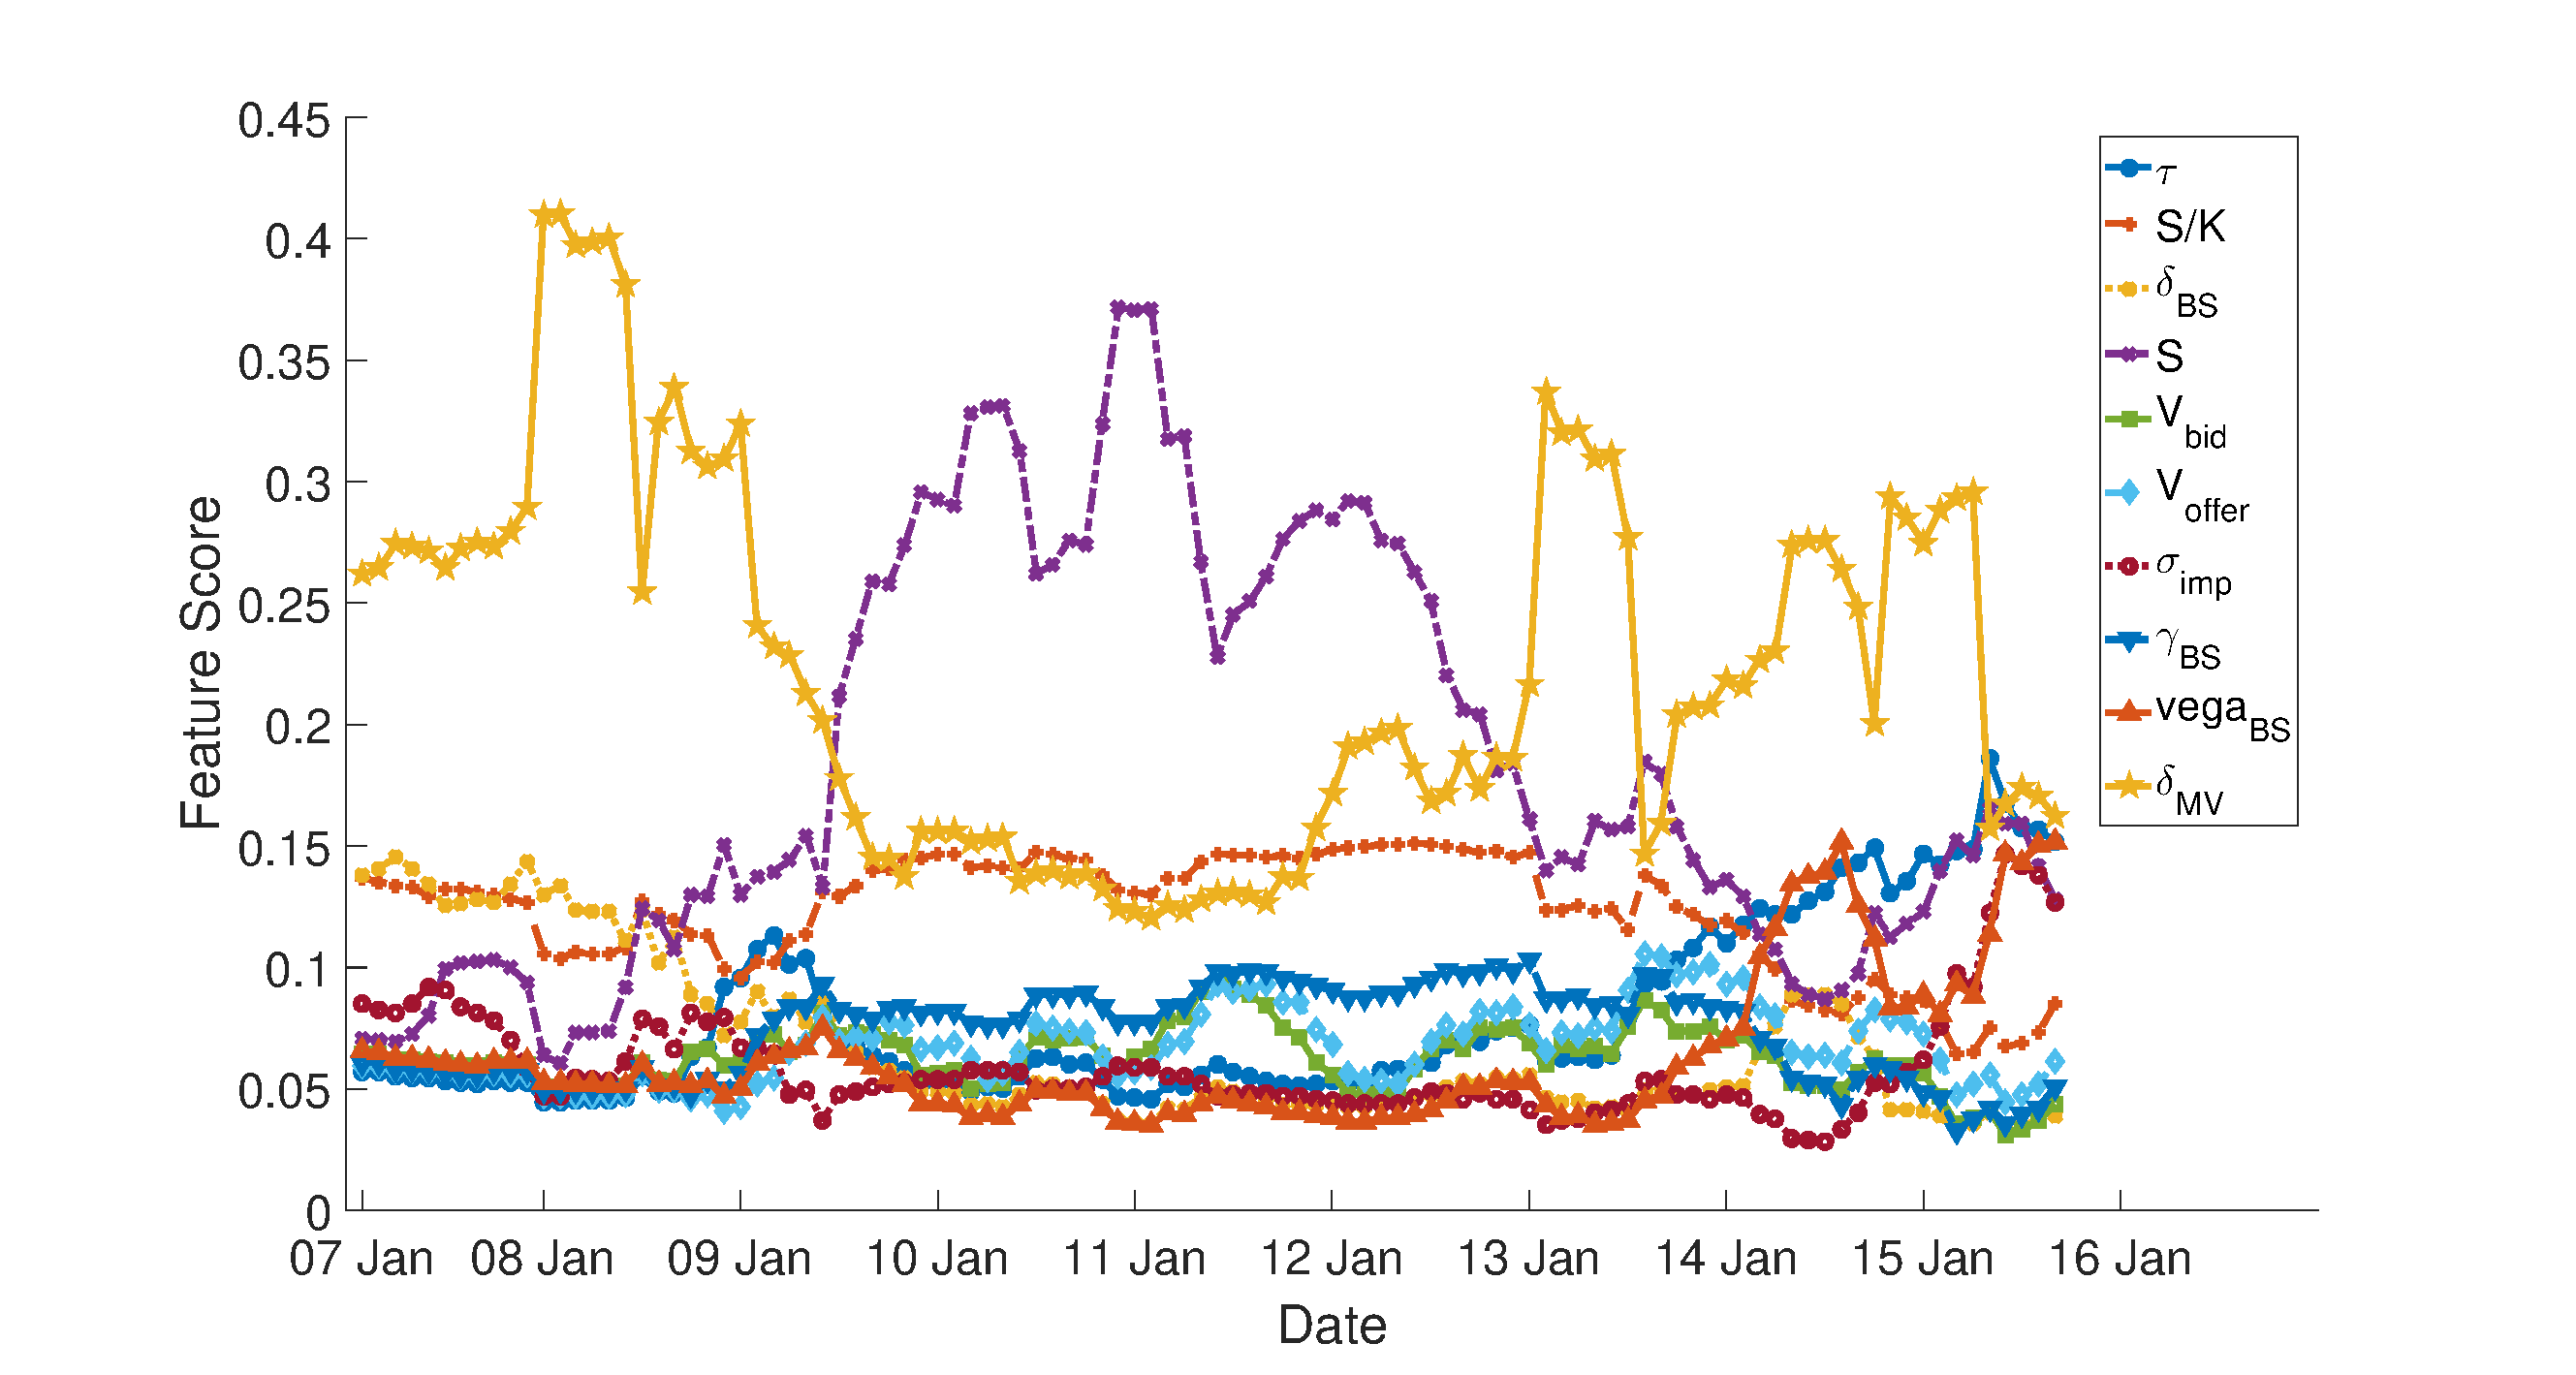
\includegraphics[width=0.90\textwidth]{CLocal0}}
  \caption{Feature Score of S\&P500 Call Option (Daily Hedging)} \label{fig:call1}
\end{figure}
\end{frame}


\begin{frame}[fragile]{Feature Score (2)}
\begin{figure}[htp]
  \centering
  \subfigure[Sequential Features ]{
    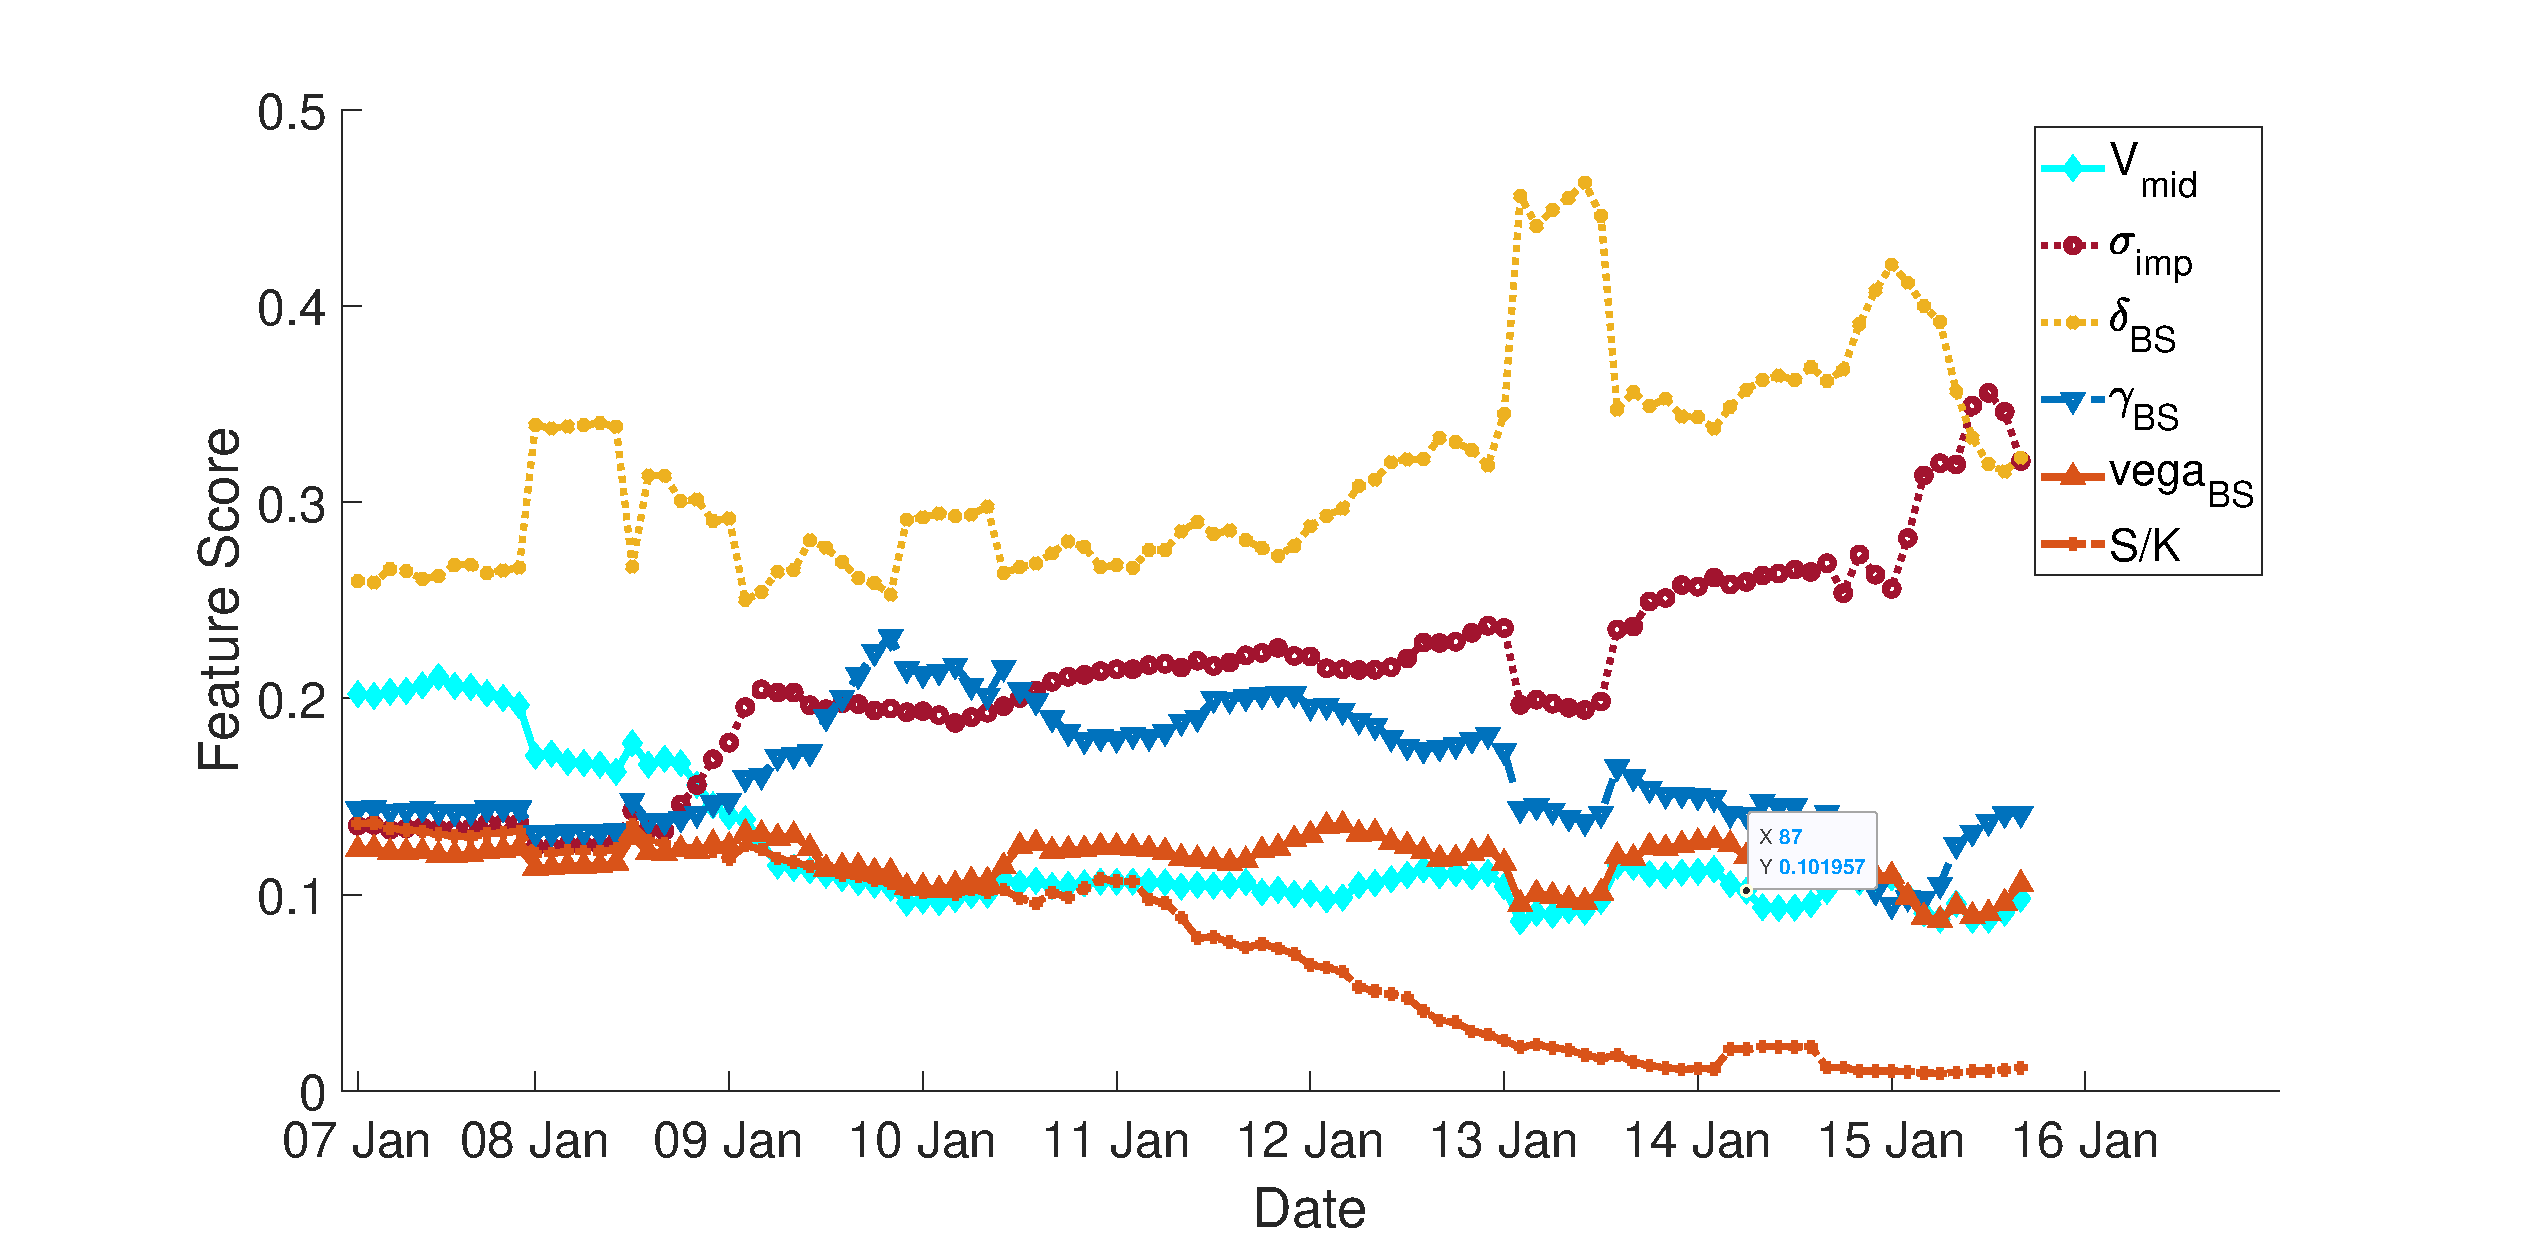
\includegraphics[width=0.90\textwidth]{C0}}
  \caption{Feature Score of S\&P500 Call Option (Daily Hedging)} \label{fig:call1}
\end{figure}
\end{frame}

\begin{frame}[fragile]{Feature Score (3)}
\begin{figure}[htp]
  \centering
  \subfigure[Local Features ]{
    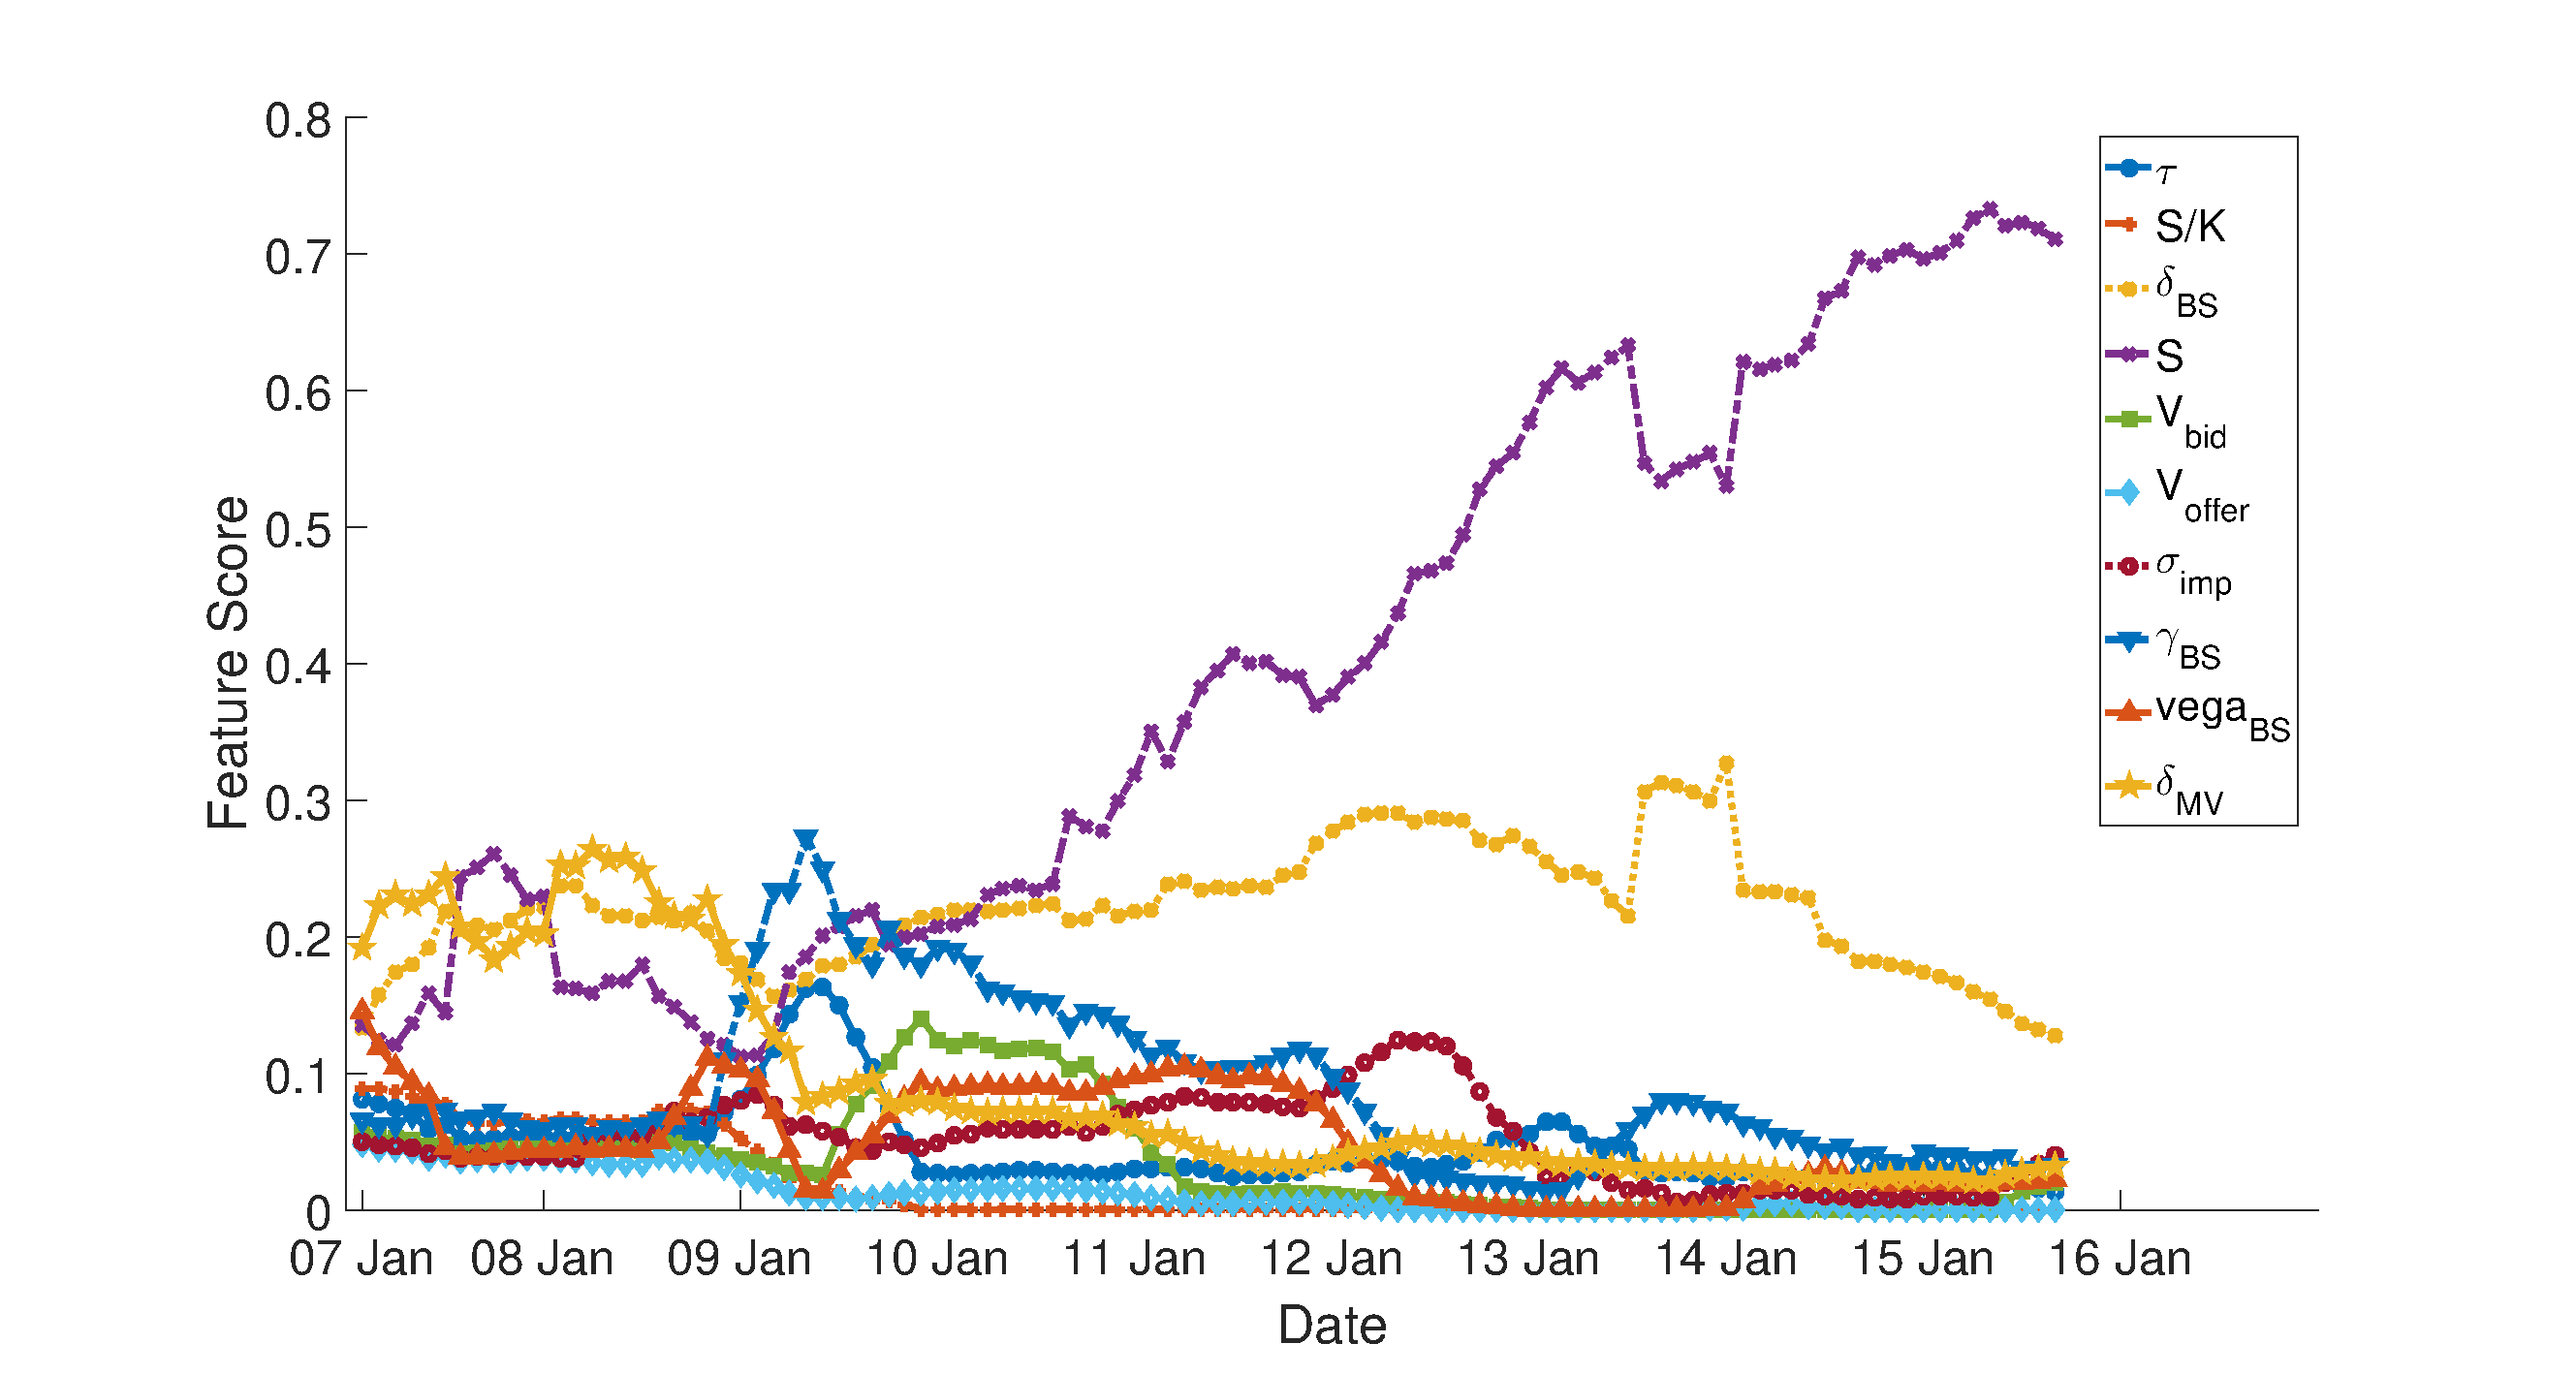
\includegraphics[width=0.90\textwidth]{CLocal1}}
  \caption{Feature Score of S\&P500 Call Option (Daily Hedging)} \label{fig:call1}
\end{figure}
\end{frame}


\begin{frame}[fragile]{Feature Score (4)}
\begin{figure}[htp]
  \centering
  \subfigure[Sequential Features ]{
    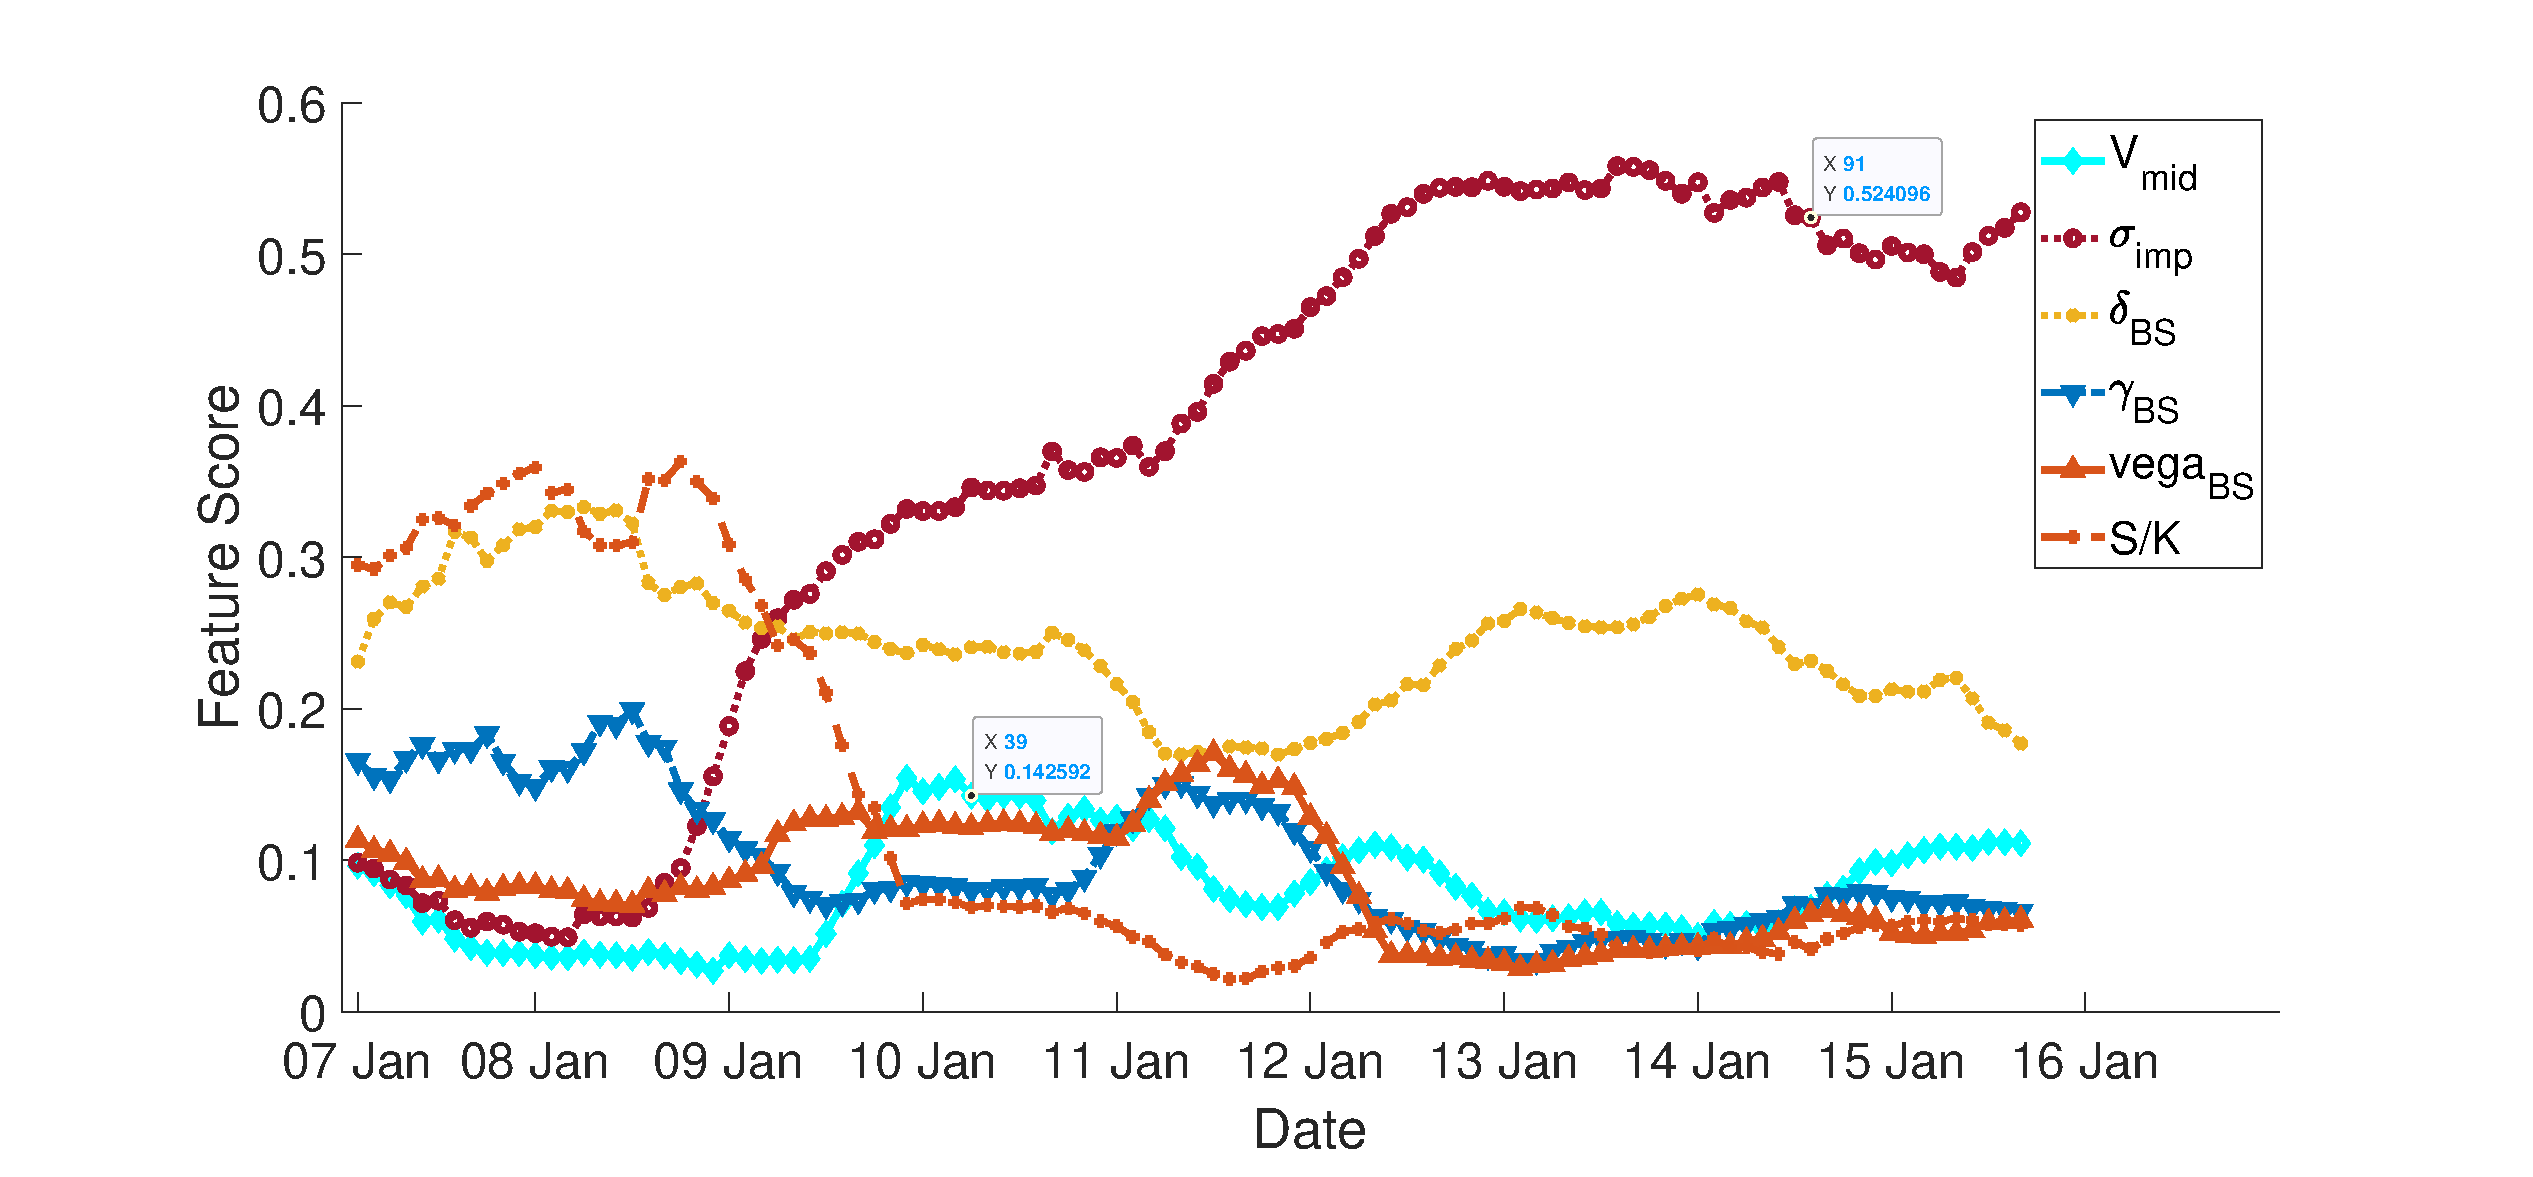
\includegraphics[width=0.90\textwidth]{C1}}
  \caption{Feature Score of S\&P500 Call Option (Daily Hedging)} \label{fig:call1}
\end{figure}
\end{frame}



\begin{frame}[fragile]{Feature Score (5)}
\begin{figure}[htp]
  \centering
  \subfigure[Local Features ]{
    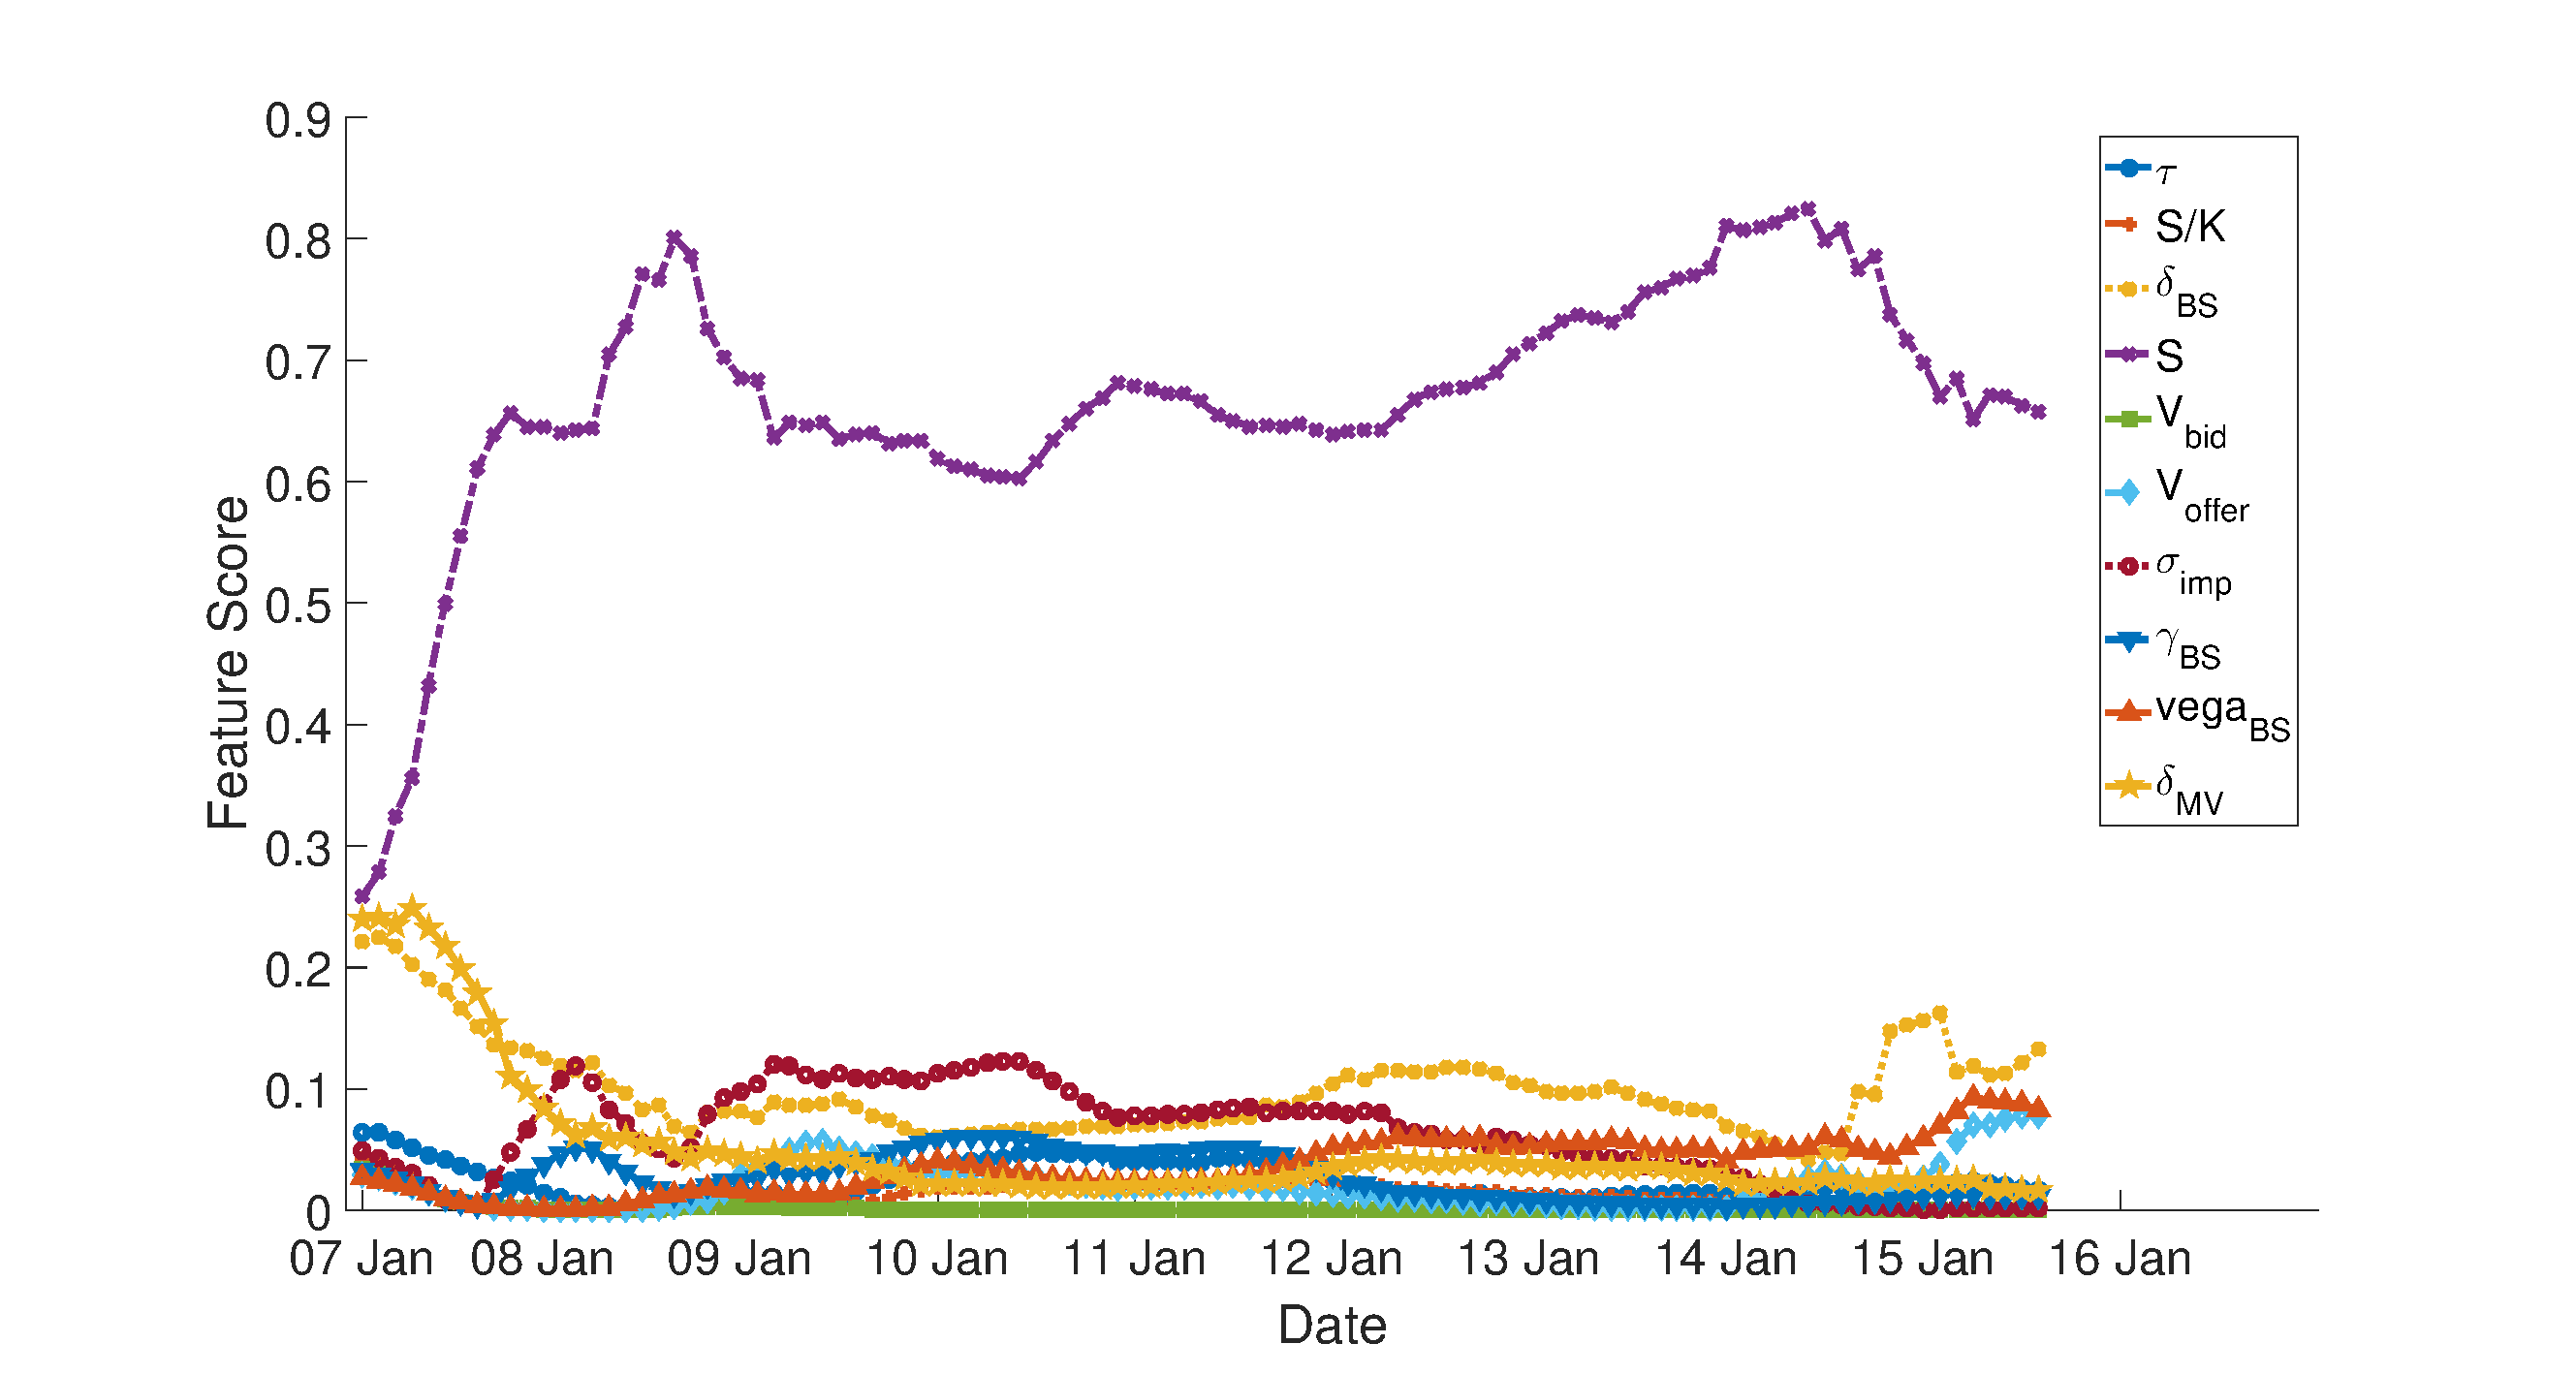
\includegraphics[width=0.90\textwidth]{CLocal2}}
  \caption{Feature Score of S\&P500 Call Option (Daily Hedging)} \label{fig:call1}
\end{figure}
\end{frame}


\begin{frame}[fragile]{Feature Score (6)}
\begin{figure}[htp]
  \centering
  \subfigure[Sequential Features ]{
    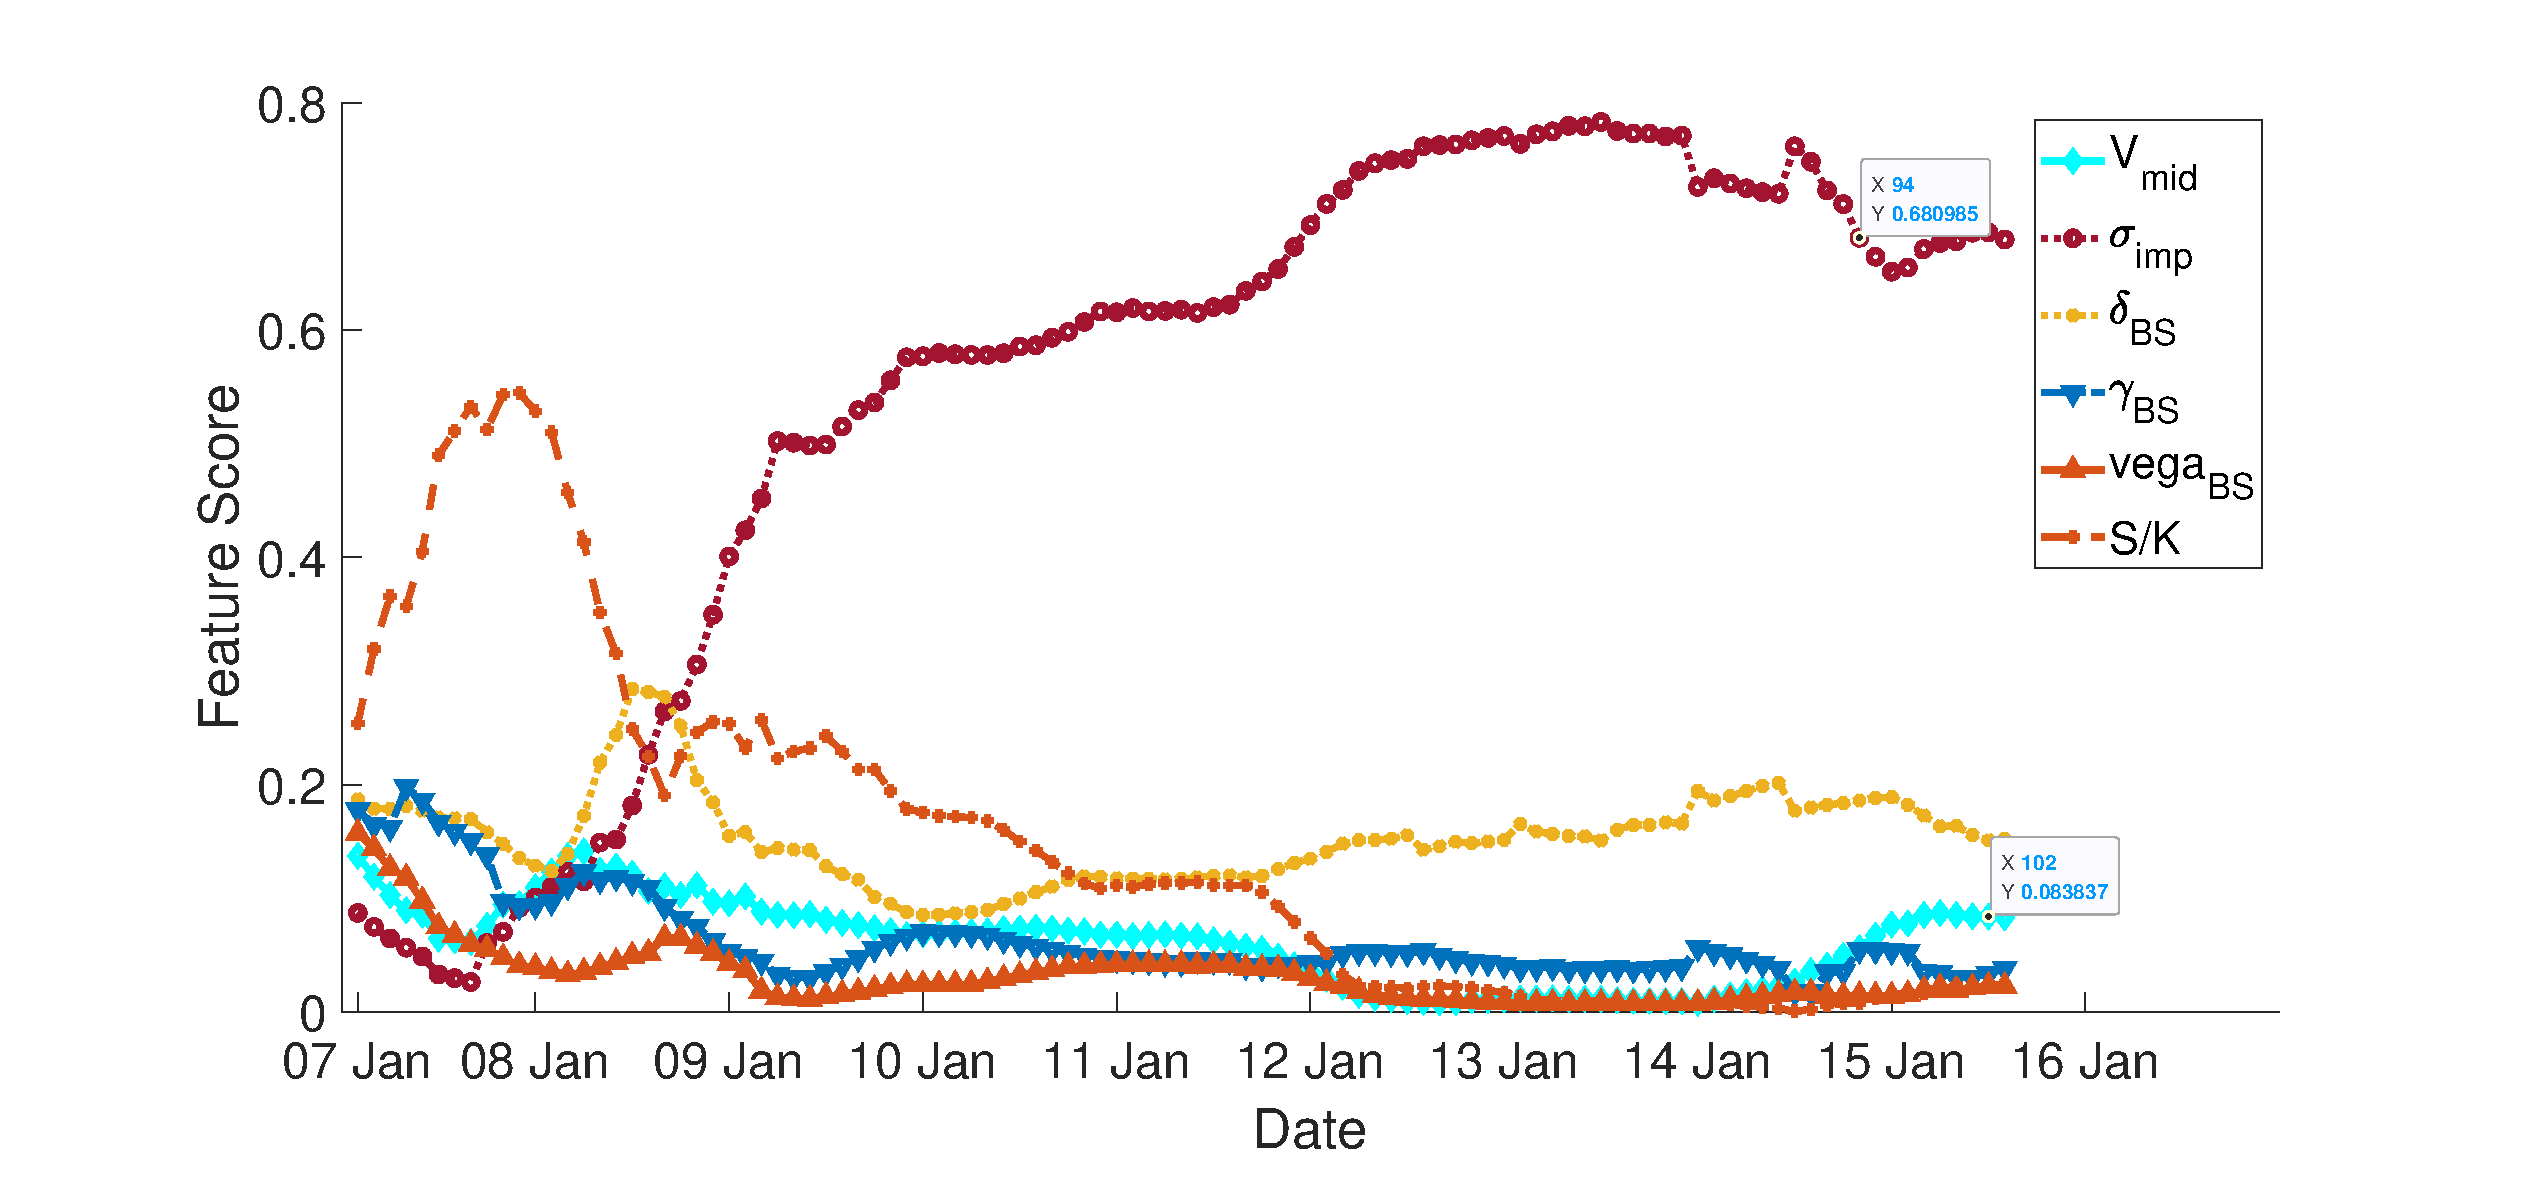
\includegraphics[width=0.90\textwidth]{C2}}
  \caption{Feature Score of S\&P500 Call Option (Daily Hedging)} \label{fig:call1}
\end{figure}
\end{frame}

\section{Summary}
\begin{frame}[fragile]{Summary}
\begin{itemize}
  \item Loosing assumption on the market dynamic is a good practise
  \item Data-driven approach can lead to better performance.
  \item Incorporating the information about the past history can further improve the hedging performance.
  \item Robust losses and robust model design are also beneficiary. 
\end{itemize}
\end{frame}

\begin{frame}{Q \& A}
  \LARGE
  \begin{quote}
    \alert{Thank you very much!}\\
    \hspace{8ex} Any Questions?
  \end{quote}
\end{frame}
\end{document}

